\documentclass[aspectratio=169,10pt]{beamer}

\usepackage[utf8]{inputenc}
\usepackage[T1]{fontenc}
\usepackage{lmodern}
\usepackage[spanish,es-nodecimaldot,es-tabla,es-noshorthands]{babel}
\usepackage{amsmath,amssymb,bm}
\usepackage{booktabs}
\usepackage{array}
\newcolumntype{L}[1]{>{\raggedright\arraybackslash}p{#1}}
\usepackage{graphicx}
\usepackage{tikz}
\usetikzlibrary{arrows.meta,positioning,calc}
\graphicspath{{../informe/figs/}{../informe/calculos/figs/}}
% identificador numerado de figuras
\newcounter{figdiap}
\newcommand{\fig}[1]{\refstepcounter{figdiap}{\footnotesize\color{tenue}\textbf{Figura~\thefigdiap.} #1\par}}

% ---------------------------------------------------------------- estilo sobrio
\definecolor{acento}{HTML}{1F4E79}
\definecolor{texto}{HTML}{1C1C1C}
\definecolor{tenue}{HTML}{6B6B6B}
\definecolor{fondo}{HTML}{F3F3F1}
\usetheme{default}
\setbeamertemplate{navigation symbols}{}
\setbeamercolor{normal text}{fg=texto}
\setbeamercolor{structure}{fg=acento}
\setbeamercolor{frametitle}{fg=acento}
\setbeamercolor{title}{fg=acento}
\setbeamercolor{block title}{fg=white,bg=acento}
\setbeamercolor{block body}{bg=fondo}
\setbeamerfont{frametitle}{size=\Large,series=\bfseries}
\setbeamertemplate{itemize items}[circle]
\setbeamertemplate{frametitle}{\vspace*{0.6em}\insertframetitle\par\vspace*{-0.2em}{\color{acento}\rule{\textwidth}{0.4pt}}}
\setbeamertemplate{footline}{%
  \hspace{1.2em}{\color{tenue}\scriptsize Plataforma Stewart 6-SPS}\hfill
  {\color{tenue}\scriptsize\insertframenumber/\inserttotalframenumber}\hspace{1.2em}\vspace{0.6em}}
\setbeamertemplate{section in toc}[sections numbered]
\setbeamercolor{section in toc}{fg=acento}
\setbeamerfont{section in toc}{size=\normalsize}
\setbeamercolor{section in toc shaded}{fg=tenue}
\setbeamertemplate{section in toc shaded}[default][55]
% portadilla antes de cada parte: el contenido con la parte actual resaltada
\newcommand{\nombreparte}[1]{\ifcase#1\or Descripción de la plataforma\or Modelo cinemático\or Modelo dinámico\or Espacio de estados y linealización\or Cálculo de variaciones\or Control óptimo: principio de Pontryagin\or Control PID descentralizado\or Realimentación de estados y observador de Luenberger\or Resultados\fi}
\newcommand{\contenidoactual}{\large\begin{enumerate}\setlength{\itemsep}{0.3em}%
  \foreach \k in {1,...,9}{\ifnum\k=\value{section}\item[\textcolor{acento}{\textbf{\k.}}]\textcolor{acento}{\textbf{\nombreparte{\k}}}%
  \else\item[\textcolor{tenue}{\k.}]\textcolor{tenue}{\nombreparte{\k}}\fi}\end{enumerate}}
\AtBeginSection{\begin{frame}{Contenido}\contenidoactual\end{frame}}

\newcommand{\vect}[1]{\bm{#1}}
\newcommand{\T}{^{\mathsf{T}}}
\newcommand{\sk}[1]{\widetilde{#1}}
\makeatletter
\newcommand{\tabinput}[1]{\@@input #1 }
\makeatother
% pie de diapositiva con el significado de las variables (nota al pie sin numero, al fondo del cuadro)
\setbeamerfont{footnote}{size=\tiny}
\newcommand{\variables}[1]{\begingroup\renewcommand{\thefootnote}{}\footnote[frame]{\textbf{Variables:} #1}\addtocounter{footnote}{-1}\endgroup}
% resultado destacado y valores numericos de la plataforma
\newcommand{\resultado}[1]{\par\smallskip\begin{beamercolorbox}[rounded=true,sep=0.45em,center]{block body}#1\end{beamercolorbox}\par\smallskip}
\newcommand{\valores}{{\color{acento}\textbf{En la plataforma:}}\ }
% Generado por scripts/generar_datos_calculo.py; no editar a mano
\newcommand{\Ts}{2}
\newcommand{\Fmax}{50}
\newcommand{\Fzero}{4.779}
\newcommand{\MzeroMat}{2.7802 & 0 & 0 & 0 & -0.0003 & 0 \\ 0 & 2.7802 & 0 & 0.0003 & 0 & 0 \\ 0 & 0 & 2.7261 & 0 & 0 & 0 \\ 0 & 0.0003 & 0 & 0.0169 & 0 & 0 \\ -0.0003 & 0 & 0 & 0 & 0.0169 & 0 \\ 0 & 0 & 0 & 0 & 0 & 0.0346}
\newcommand{\MzeroEigs}{0.0169,\allowbreak\ 0.0169,\allowbreak\ 0.0346,\allowbreak\ 2.7261,\allowbreak\ 2.7802,\allowbreak\ 2.7802}
\newcommand{\MzeroEigMin}{0.0169}
\newcommand{\AtwoOneMat}{41.00 & 0 & 0 & 0 & -0.23 & 0 \\ 0 & 41.00 & 0 & 0.23 & 0 & 0 \\ 0 & 0 & 5.74 & 0 & 0 & 0 \\ 0 & 37.89 & 0 & 17.22 & 0 & 0 \\ -37.89 & 0 & 0 & 0 & 17.22 & 0 \\ 0 & 0 & 0 & 0 & 0 & 58.09}
\newcommand{\BtwoMat}{-0.097 & -0.097 & 0.097 & 0 & 0 & 0.097 \\ -0.056 & 0.056 & -0.056 & -0.111 & 0.111 & 0.056 \\ 0.349 & 0.349 & 0.349 & 0.349 & 0.349 & 0.349 \\ -4.966 & 4.966 & 6.786 & 1.820 & -1.820 & -6.786 \\ -4.969 & -4.969 & -1.816 & 6.785 & 6.785 & -1.816 \\ -1.080 & 1.080 & -1.080 & 1.080 & -1.080 & 1.080}
\newcommand{\PolosLA}{\pm7.62,\allowbreak\ \pm6.43\ (\times2),\allowbreak\ \pm4.11\ (\times2),\allowbreak\ \pm2.40}
\newcommand{\SigmaMax}{7.62}
\newcommand{\EigAtwoOne}{58.09,\allowbreak\ 41.36,\allowbreak\ 41.36,\allowbreak\ 16.85,\allowbreak\ 16.85,\allowbreak\ 5.74}
\newcommand{\LamEigs}{0.398,\allowbreak\ 0.398,\allowbreak\ 0.502,\allowbreak\ 4.124,\allowbreak\ 10.371,\allowbreak\ 10.371}
\newcommand{\KlEigs}{427.8,\allowbreak\ 427.8,\allowbreak\ 239.6,\allowbreak\ 6.7,\allowbreak\ 6.7,\allowbreak\ 2.9}
\newcommand{\KlMax}{427.8}
\newcommand{\mLeg}{4.3607}
\newcommand{\kLeg}{185.26}
\newcommand{\mEff}{0.8054}
\newcommand{\sigmaLeg}{6.518}
\newcommand{\cLeg}{1.0000850}
\newcommand{\gLeg}{4.5865\times10^{-7}}
\newcommand{\zUnst}{1.013121}
\newcommand{\zSt}{0.987049}
\newcommand{\MxTheta}{2.94\times10^{-4}}
\newcommand{\muMulti}{1.84\times10^{-6}}
\newcommand{\omegaMulti}{1.9986,\allowbreak\ 1.9986,\allowbreak\ 2.0000,\allowbreak\ 2.0000,\allowbreak\ 2.0014,\allowbreak\ 2.0014}
\newcommand{\MdiagPlat}{2 & 2 & 2 & 0.01125 & 0.01125 & 0.0225}
\newcommand{\MdiagPatas}{0.7802 & 0.7802 & 0.7261 & 0.0057 & 0.0057 & 0.0121}
\newcommand{\KpOpt}{4556.7}
\newcommand{\KiOpt}{18445.7}
\newcommand{\KdOpt}{105.43}
\newcommand{\spOpt}{0.759}
\newcommand{\siOpt}{3.074}
\newcommand{\sdOpt}{0.703}
\newcommand{\TiOpt}{0.247}
\newcommand{\TdOpt}{23.14}
\newcommand{\JpidOpt}{4.777}
\newcommand{\alphaD}{0.7261}
\newcommand{\Dcoef}{136.93}
\newcommand{\nTwo}{18992.4}
\newcommand{\nOne}{-36700.1}
\newcommand{\nZero}{17717.8}
\newcommand{\wcPid}{187.9}
\newcommand{\PMPid}{41.6}
\newcommand{\GMPid}{11.1}
\newcommand{\MsPid}{2.15}
\newcommand{\wcHand}{37.6}
\newcommand{\GwcMag}{1.577\times10^{-4}}
\newcommand{\GwcAng}{-182.2}
\newcommand{\CwcMag}{6343}
\newcommand{\CwcAng}{+31.0}
\newcommand{\PMhand}{28.8}
\newcommand{\RouthA}{105.43}
\newcommand{\RouthB}{4371.4}
\newcommand{\RouthC}{18445.7}
\newcommand{\RouthL}{460870}
\newcommand{\RouthR}{80437}
\newcommand{\RootsCont}{-9.77 \pm 28.57j,\allowbreak\ -4.64}
\newcommand{\charPoly}{z^4 -3.7176z^3 +5.1706z^2 -3.1873z +0.7343}
\newcommand{\charRoots}{0.9907,\allowbreak\ 0.9759 \pm 0.0620j,\allowbreak\ 0.7751}
\newcommand{\rhoSiso}{0.9907}
\newcommand{\rhoPid}{0.9945}
\newcommand{\KpBase}{6000}
\newcommand{\KiBase}{6000}
\newcommand{\KdBase}{150}
\newcommand{\alphaOpt}{3.357}
\newcommand{\betaOpt}{0.3525}
\newcommand{\JssOpt}{3.633}
\newcommand{\PoloCtrl}{-85.60 \pm 30.21j}
\newcommand{\PoloObs}{-27.49 \pm 6.34j}
\newcommand{\tsCtrl}{47}
\newcommand{\cofErr}{2.2\times10^{-16}}
\newcommand{\sepErr}{1.3\times10^{-13}}
\newcommand{\normK}{8.75\times10^{4}}
\newcommand{\rhoSS}{0.9696}
\newcommand{\rhoCtrlBlock}{0.9696}
\newcommand{\obsPoleErr}{5.2\times10^{-15}}
\newcommand{\obsZmax}{0.9465}
\newcommand{\LdPos}{0.104 y 0.132}
\newcommand{\LdVel}{1.585 y 2.598}
\newcommand{\aOnda}{2}
\newcommand{\TOnda}{2.5}
\newcommand{\fOnda}{0.2}
\newcommand{\wOnda}{1.2566}
\newcommand{\AOnda}{15}
\newcommand{\rzZero}{15.000}
\newcommand{\kappaOnda}{0.7170}
\newcommand{\EOnda}{6.738\times10^{-3}}
\newcommand{\TPre}{1}
\newcommand{\rzT}{-15.000}
\newcommand{\drzZero}{0.000}
\newcommand{\drzT}{0.000}
\newcommand{\CUnoA}{-10.8273}
\newcommand{\CDosA}{10.8273}
\newcommand{\xZeroA}{0.000}
\newcommand{\xTA}{0.000}
\newcommand{\JA}{393.7}
\newcommand{\CUnoB}{-10.7539}
\newcommand{\CDosB}{-0.0725}
\newcommand{\xZeroB}{0.000}
\newcommand{\xTB}{-10.899}
\newcommand{\JB}{274.9}
\newcommand{\CUnoC}{0.0725}
\newcommand{\CDosC}{10.7539}
\newcommand{\xZeroC}{10.899}
\newcommand{\xTC}{0.000}
\newcommand{\JC}{274.9}
\newcommand{\CUnoD}{0.0000}
\newcommand{\CDosD}{0.0000}
\newcommand{\xZeroD}{10.754}
\newcommand{\xTD}{-10.754}
\newcommand{\JD}{159.2}
\newcommand{\dlEn}{14.26}
\newcommand{\uEnMax}{17.23}
\newcommand{\EEn}{1.980\times10^{-4}}
\newcommand{\aMax}{0.08}
\newcommand{\dlTm}{23.19}
\newcommand{\TMin}{1.077}
\newcommand{\tSw}{0.538}
\newcommand{\vPico}{43.1}
\newcommand{\uBang}{64.4}
\newcommand{\VAFunoMedia}{-306.92}
\newcommand{\FITunoMedia}{-99.7}
\newcommand{\VAFdosMedia}{97.81}
\newcommand{\FITdosMedia}{84.8}
\newcommand{\FITdosMin}{80.2}
\newcommand{\FITanMedia}{84.7}
\newcommand{\IdHval}{0.1}
\newcommand{\aIdMin}{1.91977}
\newcommand{\aIdMax}{1.99607}
\newcommand{\aAn}{2.00301}
\newcommand{\mIdMin}{0.835}
\newcommand{\mIdMax}{0.900}
\newcommand{\mAn}{0.805}
\newcommand{\IdKp}{1500}
\newcommand{\IdKd}{60}
\newcommand{\IdLmin}{275.1}
\newcommand{\IdLmax}{291.7}
\newcommand{\IdSigma}{0.05}
\newcommand{\mIdDirMin}{0.105}
\newcommand{\mIdDirMax}{0.142}
\newcommand{\IdTsId}{10}
\newcommand{\IdFc}{20}
\newcommand{\IdD}{5}
\newcommand{\mErrMax}{12}

\newcommand{\RefSendl}{14.26}
\newcommand{\RefSendld}{40.33}
\newcommand{\RefSenqdd}{119.91}
\newcommand{\RefSenFff}{4.88}
\newcommand{\RefSendv}{0.00}
\newcommand{\RefSendq}{0.00}
\newcommand{\RefSenFreg}{8.84}
\newcommand{\RefSenPidRms}{0.116}
\newcommand{\RefSenPidEmax}{0.37}
\newcommand{\RefSenPidFmax}{20.6}
\newcommand{\RefSenSsRms}{0.124}
\newcommand{\RefSenSsEmax}{0.52}
\newcommand{\RefSenSsFmax}{8.8}
\newcommand{\RefSeisdl}{22.97}
\newcommand{\RefSeisdld}{39.41}
\newcommand{\RefSeisqdd}{60.45}
\newcommand{\RefSeisFff}{7.32}
\newcommand{\RefSeisdv}{0.00}
\newcommand{\RefSeisdq}{0.00}
\newcommand{\RefSeisFreg}{10.36}
\newcommand{\RefSeisPidRms}{1.424}
\newcommand{\RefSeisPidEmax}{11.99}
\newcommand{\RefSeisPidFmax}{50.0}
\newcommand{\RefSeisSsRms}{0.497}
\newcommand{\RefSeisSsEmax}{11.96}
\newcommand{\RefSeisSsFmax}{50.0}
\newcommand{\RefCircdl}{11.81}
\newcommand{\RefCircdld}{29.68}
\newcommand{\RefCircqdd}{94.75}
\newcommand{\RefCircFff}{7.05}
\newcommand{\RefCircdv}{0.00}
\newcommand{\RefCircdq}{0.00}
\newcommand{\RefCircFreg}{10.15}
\newcommand{\RefCircPidRms}{1.740}
\newcommand{\RefCircPidEmax}{14.96}
\newcommand{\RefCircPidFmax}{50.0}
\newcommand{\RefCircSsRms}{0.690}
\newcommand{\RefCircSsEmax}{14.96}
\newcommand{\RefCircSsFmax}{50.0}
\newcommand{\RefFAdl}{4.68}
\newcommand{\RefFAdld}{20.16}
\newcommand{\RefFAqdd}{59.14}
\newcommand{\RefFAFff}{4.81}
\newcommand{\RefFAdv}{21.44}
\newcommand{\RefFAdq}{0.00}
\newcommand{\RefFAFreg}{8.71}
\newcommand{\RefFAPidRms}{0.096}
\newcommand{\RefFAPidEmax}{0.32}
\newcommand{\RefFAPidFmax}{20.6}
\newcommand{\RefFASsRms}{0.071}
\newcommand{\RefFASsEmax}{0.32}
\newcommand{\RefFASsFmax}{8.7}
\newcommand{\RefFBdl}{10.36}
\newcommand{\RefFBdld}{21.09}
\newcommand{\RefFBqdd}{59.15}
\newcommand{\RefFBFff}{4.82}
\newcommand{\RefFBdv}{22.48}
\newcommand{\RefFBdq}{0.00}
\newcommand{\RefFBFreg}{8.73}
\newcommand{\RefFBPidRms}{0.097}
\newcommand{\RefFBPidEmax}{0.32}
\newcommand{\RefFBPidFmax}{20.6}
\newcommand{\RefFBSsRms}{0.073}
\newcommand{\RefFBSsEmax}{0.32}
\newcommand{\RefFBSsFmax}{8.7}
\newcommand{\RefFCdl}{10.36}
\newcommand{\RefFCdld}{21.46}
\newcommand{\RefFCqdd}{59.15}
\newcommand{\RefFCFff}{4.82}
\newcommand{\RefFCdv}{22.35}
\newcommand{\RefFCdq}{0.00}
\newcommand{\RefFCFreg}{8.71}
\newcommand{\RefFCPidRms}{0.097}
\newcommand{\RefFCPidEmax}{0.34}
\newcommand{\RefFCPidFmax}{20.6}
\newcommand{\RefFCSsRms}{0.072}
\newcommand{\RefFCSsEmax}{0.33}
\newcommand{\RefFCSsFmax}{8.7}
\newcommand{\RefFDdl}{10.23}
\newcommand{\RefFDdld}{21.18}
\newcommand{\RefFDqdd}{42.66}
\newcommand{\RefFDFff}{4.82}
\newcommand{\RefFDdv}{22.19}
\newcommand{\RefFDdq}{0.00}
\newcommand{\RefFDFreg}{8.73}
\newcommand{\RefFDPidRms}{0.098}
\newcommand{\RefFDPidEmax}{0.34}
\newcommand{\RefFDPidFmax}{20.6}
\newcommand{\RefFDSsRms}{0.073}
\newcommand{\RefFDSsEmax}{0.31}
\newcommand{\RefFDSsFmax}{8.7}
\newcommand{\RefFijdl}{23.19}
\newcommand{\RefFijdld}{46.31}
\newcommand{\RefFijqdd}{361.37}
\newcommand{\RefFijFff}{7.41}
\newcommand{\RefFijdv}{39.00}
\newcommand{\RefFijdq}{0.00}
\newcommand{\RefFijFreg}{11.53}
\newcommand{\RefFijPidRms}{0.333}
\newcommand{\RefFijPidEmax}{1.41}
\newcommand{\RefFijPidFmax}{21.7}
\newcommand{\RefFijSsRms}{0.086}
\newcommand{\RefFijSsEmax}{0.47}
\newcommand{\RefFijSsFmax}{11.5}
\newcommand{\RefTmindl}{23.19}
\newcommand{\RefTmindld}{42.99}
\newcommand{\RefTminqdd}{68.05}
\newcommand{\RefTminFff}{6.84}
\newcommand{\RefTmindv}{0.00}
\newcommand{\RefTmindq}{0.00}
\newcommand{\RefTminFreg}{10.21}
\newcommand{\RefTminPidRms}{0.306}
\newcommand{\RefTminPidEmax}{0.88}
\newcommand{\RefTminPidFmax}{21.6}
\newcommand{\RefTminSsRms}{0.083}
\newcommand{\RefTminSsEmax}{0.22}
\newcommand{\RefTminSsFmax}{10.2}
\newcommand{\RefCurvadl}{14.26}
\newcommand{\RefCurvadld}{40.33}
\newcommand{\RefCurvaqdd}{119.91}
\newcommand{\RefCurvaFff}{4.88}
\newcommand{\RefCurvadv}{34.59}
\newcommand{\RefCurvadq}{19.24}
\newcommand{\RefCurvaFreg}{50.00}
\newcommand{\RefCurvaPidRms}{0.605}
\newcommand{\RefCurvaPidEmax}{19.05}
\newcommand{\RefCurvaPidFmax}{50.0}
\newcommand{\RefCurvaSsRms}{0.634}
\newcommand{\RefCurvaSsEmax}{19.20}
\newcommand{\RefCurvaSsFmax}{50.0}


\title{Modelado, identificación y control de una plataforma Stewart 6-SPS}
\author{Santiago Alejandro Zúñiga Melo}
\institute{Maestría en Ingeniería Electrónica\\Escuela Colombiana de Ingeniería Julio Garavito\\[0.4em]
Estrategias Óptimas de Control --- Prof. Jorge Andrés Puerto Acosta, Ph.D.}
\date{}

\begin{document}

\begin{frame}[plain]
\titlepage
\end{frame}

\begin{frame}{Objetivo y contenido}
\resultado{\textbf{Objetivo general del proyecto:} Diseñar, analizar, implementar y comparar estrategias clásicas, modernas y óptimas de control para la posición y la orientación de una plataforma Stewart 6-SPS.}
\vspace{-0.3em}
{\small\textbf{Alcance de la primera entrega:} modelo cinemático y dinámico, identificación, trayectorias óptimas y las dos primeras estrategias de control, PID descentralizado y realimentación de estados con observador de Luenberger.\par}
\medskip
\begin{columns}[T]
\column{0.48\textwidth}
\begin{enumerate}
\setlength{\itemsep}{0.1em}
\item Descripción de la plataforma
\item Modelo cinemático
\item Modelo dinámico
\item Espacio de estados y linealización
\item Cálculo de variaciones
\end{enumerate}
\column{0.48\textwidth}
\begin{enumerate}
\setcounter{enumi}{5}
\setlength{\itemsep}{0.1em}
\item Control óptimo: principio de Pontryagin
\item Control PID descentralizado
\item Realimentación de estados y observador de Luenberger
\item Resultados
\end{enumerate}
\end{columns}
\end{frame}

% ===================================================================================================
\section{Descripción de la plataforma}

\begin{frame}{La plataforma Stewart 6-SPS}
\begin{columns}[c]
\column{0.40\textwidth}
\centering
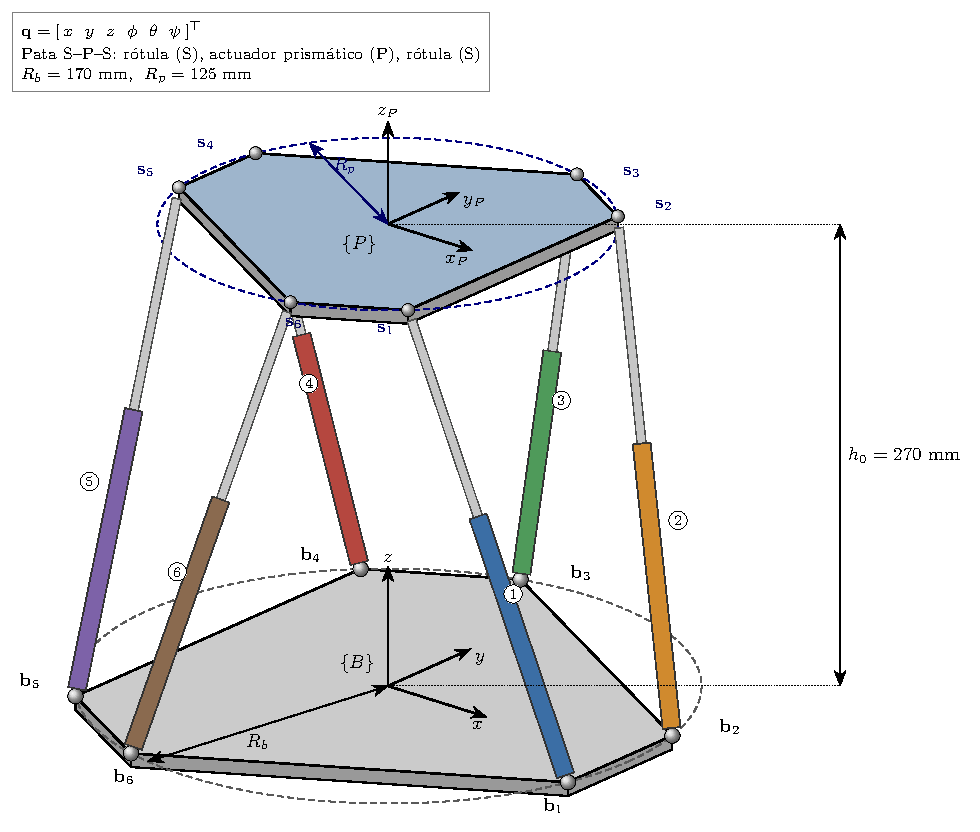
\includegraphics[width=\linewidth]{arquitectura_6sps.pdf}\\
\fig{Arquitectura 6-SPS con la geometría y la vista del simulador}
\column{0.57\textwidth}
\begin{itemize}
\setlength{\itemsep}{0.6em}
\item Base fija $\{B\}$, plataforma móvil $\{P\}$ y seis patas S--P--S
\item Cada pata: cilindro unido a $B_i$, pistón unido a $P_i$ y actuador lineal; su entrada es la \textbf{fuerza axial} $F_i$ (modelo del momento generalizado)
\item Seis longitudes controlan seis grados de libertad: $\vect q = [x\ y\ z\ \phi\ \theta\ \psi]\T$
\item Sistema MIMO acoplado y no lineal
\end{itemize}
\end{columns}
\variables{$\{B\}$: marco de la base; $\{P\}$: marco de la plataforma; $B_i$, $P_i$: anclajes de la pata $i$ en la base y en la plataforma; $F_i$: fuerza axial del actuador $i$ [N]; $\vect q$: posición y orientación; $x, y, z$: posición del centro de la plataforma [m]; $\phi, \theta, \psi$: alabeo, cabeceo y guiñada [rad].}
\end{frame}

\begin{frame}{Parámetros}
\begin{columns}[T]
\column{0.46\textwidth}
\centering
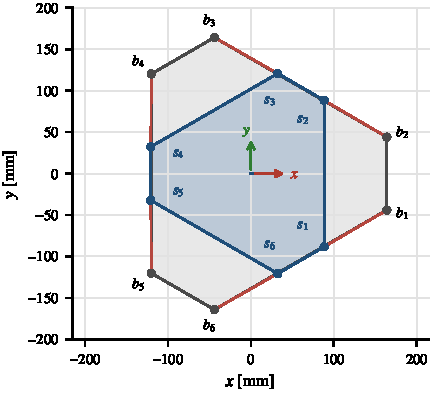
\includegraphics[width=\linewidth,height=0.62\textheight,keepaspectratio]{geometria.pdf}\\
\fig{Anclajes de la base y de la plataforma}
\column{0.52\textwidth}
\footnotesize
\begin{tabular}{@{}lr@{}}
\toprule
Parámetro & Valor \\
\midrule
$R_b$ / $R_p$ & 170 / 125 mm \\
$h_0$ / $l_0$ & 270 / 283.93 mm \\
$m_P$ & 2.0 kg \\
$m_C$, $b_C$ (cilindro) & 0.45 kg, 80 mm \\
$m_S$, $b_S$ (pistón) & 0.12 kg, 50 mm \\
Carrera de cada pata & 100 mm \\
$F_{\max}$ (fuerza por actuador) & $\pm\Fmax$ N \\
$\ddot l_{\max}$ (restricción) & 0.08 m/s$^2$ \\
$T_s$ & \Ts{} ms \\
\bottomrule
\end{tabular}
\end{columns}
\variables{$R_b$, $R_p$: radios de los anclajes de base y plataforma; $h_0$: altura nominal; $l_0$: longitud nominal de pata; $m_P$, $m_C$, $m_S$: masas de plataforma, cilindro y pistón; $b_C$, $b_S$: distancia de $B_i$ al centro de masa del cilindro y de $P_i$ al del pistón; $F_{\max}$: fuerza máxima por actuador; $\ddot l_{\max}$: aceleración máxima de pata; $T_s$: periodo de muestreo.}
\end{frame}

% ===================================================================================================

\section{Modelo cinemático}

\begin{frame}{Posición y orientación}
\small
La orientación se describe con tres giros sucesivos Z--Y--X: $\psi$ sobre $\vect z$, $\theta$ sobre el eje $\vect y$ girado y $\phi$ sobre el eje $\vect x$ resultante.
\[
\vect R = \vect R_z(\psi)\vect R_y(\theta)\vect R_x(\phi) =
\begin{bmatrix}
c_\psi c_\theta & c_\psi s_\theta s_\phi - s_\psi c_\phi & c_\psi s_\theta c_\phi + s_\psi s_\phi\\
s_\psi c_\theta & s_\psi s_\theta s_\phi + c_\psi c_\phi & s_\psi s_\theta c_\phi - c_\psi s_\phi\\
-s_\theta & c_\theta s_\phi & c_\theta c_\phi
\end{bmatrix}
\]
La velocidad angular es la suma de las tres rotaciones elementales, no la derivada de los ángulos:
\[
\vect\omega = \dot\psi\hat{\vect z} + \dot\theta\,\vect R_z\hat{\vect y} + \dot\phi\,\vect R_z\vect R_y\hat{\vect x} = \vect E\begin{bmatrix}\dot\phi\\ \dot\theta\\ \dot\psi\end{bmatrix},
\qquad
\vect E = \begin{bmatrix}c_\psi c_\theta & -s_\psi & 0\\ s_\psi c_\theta & c_\psi & 0\\ -s_\theta & 0 & 1\end{bmatrix}
\]
\resultado{$\displaystyle \vect\nu = \begin{bmatrix}\vect v\\ \vect\omega\end{bmatrix} = \vect T\dot{\vect q},\qquad \vect T = \begin{bmatrix}\vect I & \vect 0\\ \vect 0 & \vect E\end{bmatrix},\qquad \vect T_0 = \vect I_6\ \text{en la configuración nominal}$}
\variables{$\vect R$: matriz de rotación de $\{P\}$ respecto a $\{B\}$; $\vect R_x, \vect R_y, \vect R_z$: rotaciones elementales; $c_\alpha = \cos\alpha$, $s_\alpha = \sin\alpha$; $\phi, \theta, \psi$: alabeo, cabeceo y guiñada; $\vect\omega$: velocidad angular de la plataforma en $\{B\}$; $\hat{\vect x}, \hat{\vect y}, \hat{\vect z}$: ejes unitarios; $\vect E$: matriz que pasa de derivadas de ángulos a $\vect\omega$; $\vect v$: velocidad del centro; $\vect\nu$: twist $[\vect v; \vect\omega]$; $\vect T$: matriz $\vect\nu = \vect T\dot{\vect q}$; $\dot{\vect q}$: derivada de la posición y la orientación.}
\end{frame}

\begin{frame}{Cinemática inversa: lazo vectorial}
\begin{columns}[c]
\column{0.52\textwidth}
\small
Al extremo $P_i$ se llega por la pata o por la plataforma:
\[
\vect b_i + \vect l_i = \vect p + \vect R\vect s_i
\]
\resultado{$\displaystyle l_i = \lVert\vect p + \vect R\vect s_i - \vect b_i\rVert,\qquad \hat{\vect l}_i = \frac{\vect l_i}{l_i}$}
\valores pata 1 en la configuración nominal
\begin{align*}
\vect l_1 &= (88.39 - 164.21,\ -88.39 + 44.00,\ 270)\\
&= (-75.82,\ -44.39,\ 270)\ \text{mm}\\
l_1 &= \sqrt{5748.7 + 1970.5 + 72900} = 283.93\ \text{mm}\\
\hat{\vect l}_1 &= (-0.2670,\ -0.1563,\ 0.9509)
\end{align*}
Solución única y explícita.
\column{0.44\textwidth}
\centering
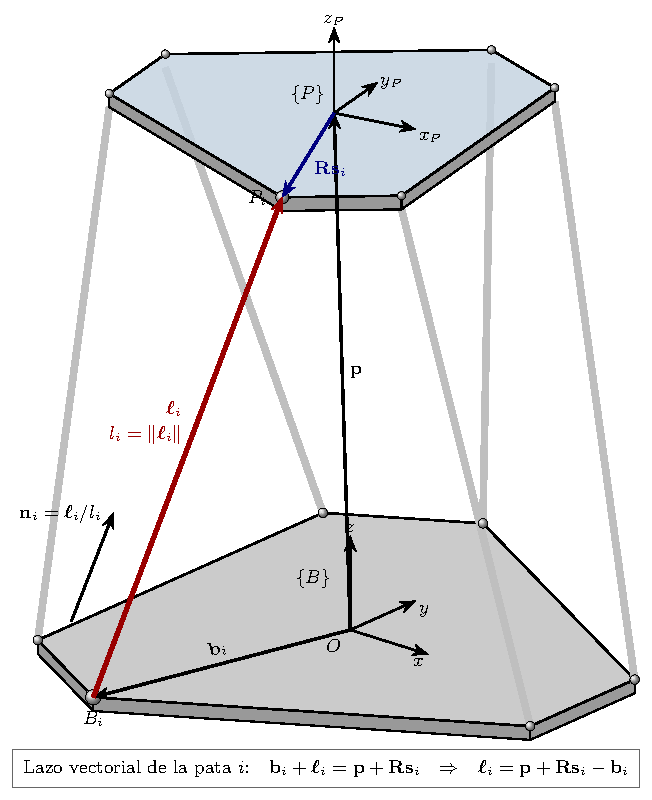
\includegraphics[height=0.6\textheight,keepaspectratio]{lazo_vectorial_pata.pdf}\\
\fig{Lazo vectorial de una pata}
\end{columns}
\variables{$\vect b_i$: anclaje de la pata $i$ en la base; $\vect s_i$: anclaje en la plataforma (marco $\{P\}$); $\vect p$: posición del centro de la plataforma; $\vect R$: rotación; $\vect l_i$: vector de la pata (de $B_i$ a $P_i$); $l_i$: longitud de la pata; $\hat{\vect l}_i$: vector unitario de la pata.}
\end{frame}

\begin{frame}{Cinemática diferencial: Jacobiano}
\small
\begin{columns}[T]
\column{0.53\textwidth}
\textbf{Velocidad de alargamiento de la pata $i$}
\begin{align*}
l_i^2 = \vect l_i\T\vect l_i \quad&\Rightarrow\quad \dot l_i = \hat{\vect l}_i\T\dot{\vect l}_i\\
\dot{\vect l}_i &= \vect v + \vect\omega\times\vect p_i,\qquad \vect p_i = \vect R\vect s_i\\
\hat{\vect l}_i\T(\vect\omega\times\vect p_i) &= (\vect p_i\times\hat{\vect l}_i)\T\vect\omega
\end{align*}
\textbf{Dualidad estática}
\[
\vect F\T\dot{\vect l} = \vect w\T\vect\nu\quad\forall\,\vect\nu
\quad\Rightarrow\quad
\vect w = \vect J\T\vect F
\]
\column{0.43\textwidth}
\resultado{$\displaystyle \dot{\vect l} = \vect J\vect\nu = \vect J\vect T\dot{\vect q}$\\[0.5em]
$\displaystyle \vect J_i = \begin{bmatrix}\hat{\vect l}_i\T & (\vect p_i\times\hat{\vect l}_i)\T\end{bmatrix}$}
\valores
\begin{itemize}
\setlength{\itemsep}{0.2em}
\item $\sigma(\vect J_0) = \{2.33,\ 0.54,\ 0.54,\ 0.20,\ 0.20,\ 0.09\}$
\item $\kappa(\vect J_0) = 25.4$, y $\kappa \le 27.4$ en todo el espacio de trabajo
\item Lejos de singularidades
\end{itemize}
\end{columns}
\variables{$l_i$, $\dot l_i$: longitud de la pata y su velocidad; $\vect l_i$: vector de la pata; $\hat{\vect l}_i$: su vector unitario; $\vect p_i = \vect R\vect s_i$: anclaje superior respecto al centro, en $\{B\}$; $\vect v$, $\vect\omega$: velocidad lineal y angular de la plataforma; $\vect\nu$: twist; $\vect J$: Jacobiano; $\vect T$: transformación de $\dot{\vect q}$ a $\vect\nu$; $\vect F$: fuerzas de las patas; $\vect w$: fuerza y momento sobre la plataforma; $\sigma$: valores singulares; $\kappa$: número de condición.}
\end{frame}

% ===================================================================================================
\section{Modelo dinámico}

\begin{frame}{Principio de Hamilton y ecuaciones de Euler--Lagrange}
\small
\textbf{Principio de Hamilton.} La trayectoria real hace estacionaria la acción $\mathcal J[\vect q] = \int_{t_0}^{t_f}L\,dt$, con $L = \mathcal T - \mathcal V$ y $\delta\vect q(t_0) = \delta\vect q(t_f) = \vect 0$. Integrando por partes:
\[
\delta\mathcal J = \underbrace{\Big[L_{\dot{\vect q}}\T\delta\vect q\Big]_{t_0}^{t_f}}_{=\,0} + \int_{t_0}^{t_f}\Big(L_{\vect q} - \tfrac{d}{dt}L_{\dot{\vect q}}\Big)\T\delta\vect q\,dt = 0
\quad\Rightarrow\quad
\frac{d}{dt}\frac{\partial L}{\partial\dot{\vect q}} - \frac{\partial L}{\partial\vect q} = \vect 0
\]
\textbf{Ecuación de movimiento.} Con las fuerzas $\vect Q$ de actuadores y perturbaciones, sin disipación, y $\mathcal T = \tfrac12\dot{\vect q}\T\vect M(\vect q)\dot{\vect q}$:
\[
\frac{d}{dt}\frac{\partial\mathcal T}{\partial\dot{\vect q}} - \frac{\partial\mathcal T}{\partial\vect q} + \frac{\partial\mathcal V}{\partial\vect q} = \vect Q
\]
\resultado{$\displaystyle \vect M(\vect q)\ddot{\vect q} + \vect C(\vect q, \dot{\vect q})\dot{\vect q} + \vect g(\vect q) = (\vect J\vect T)\T\vect F + \vect\tau_d$}
\[
\vect C\dot{\vect q} = \dot{\vect M}\dot{\vect q} - \tfrac12\frac{\partial}{\partial\vect q}\big(\dot{\vect q}\T\vect M\dot{\vect q}\big),\qquad \vect g = \frac{\partial\mathcal V}{\partial\vect q}
\]
\variables{$\mathcal J$: funcional (acción); $L = \mathcal T - \mathcal V$: lagrangiano; $\mathcal T$, $\mathcal V$: energía cinética y potencial; $\delta\vect q$: variación de la trayectoria; $L_{\vect q}$, $L_{\dot{\vect q}}$: derivadas parciales de $L$; $\vect Q$: fuerzas no conservativas; $\vect M$: matriz de inercia; $\vect C\dot{\vect q}$: términos de Coriolis y centrífugos; $\vect g$: vector de fuerzas gravitacionales generalizadas; $\vect\tau_d$: perturbación externa.}
\end{frame}

\begin{frame}{Método del momento generalizado}
\begin{columns}[c]
\column{0.49\textwidth}
\footnotesize
Para cada cuerpo rígido $c$ con velocidad $\vect u_c = \vect J_c\vect\nu$:
\[
\vect q_c = \vect I_c\vect u_c,\qquad {}^P\vect f_c = \vect J_c\T\frac{d}{dt}\left(\vect I_c\vect J_c\vect T\dot{\vect q}\right)
\]
\textbf{Cilindro}, con centro a $b_C$ de $B_i$:
\[
\dot{\vect p}_{C_i} = \vect\omega_{l_i}\times b_C\hat{\vect l}_i \quad\Rightarrow\quad \vect J_{B_i} = b_C\sk{\hat{\vect l}}_i\T\vect J_{D_i}
\]
\textbf{Pistón}, con centro a $b_S$ de $P_i$:
\[
\vect J_{G_i} = \left(\vect I - b_S\sk{\hat{\vect l}}_i\T\sk{\bar{\vect l}}_i\right)\begin{bmatrix}\vect I & \sk{\vect p}_i\T\end{bmatrix}
\]
\textbf{Rotación} de ambos con el giro de la pata, $\vect\omega_{l_i} = \dfrac{\vect l_i\times\dot{\vect l}_i}{\vect l_i\T\vect l_i} = \vect J_{D_i}\vect\nu$, e inercia axisimétrica:
\[
\vect I|_B = I_\parallel\hat{\vect l}\hat{\vect l}\T + I_\perp\big(\vect I - \hat{\vect l}\hat{\vect l}\T\big)
\]
\column{0.48\textwidth}
\centering
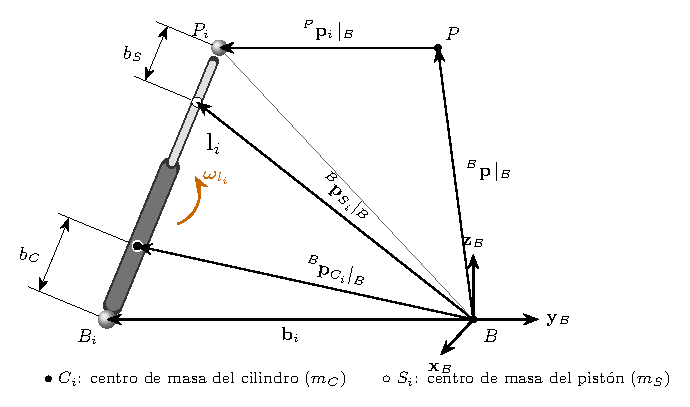
\includegraphics[width=\linewidth]{cuerpos_pata.pdf}\\
\fig{Cuerpos de la pata $i$ y vectores de posición en $\{B\}$}
\end{columns}
\variables{$c$: cuerpo rígido (plataforma, cilindro o pistón); $\vect u_c$: velocidad del cuerpo (lineal y angular); $\vect J_c$: su Jacobiano respecto al twist $\vect\nu$; $\vect I_c$: matriz de inercia (masa e inercia rotacional); $\vect q_c$: momento generalizado; ${}^P\vect f_c$: fuerza que el cuerpo transmite a la plataforma; $\vect p_{C_i}$: centro de masa del cilindro; $\vect J_{B_i}$, $\vect J_{G_i}$: Jacobianos de los centros de masa de cilindro y pistón; $b_C$, $b_S$: posiciones de los centros de masa; $I_\parallel$, $I_\perp$: inercias axial y transversal; $\vect\omega_{l_i}$: velocidad angular de la pata; $\vect J_{D_i}$: su Jacobiano.}
\end{frame}

\begin{frame}{Matriz de inercia, Coriolis y fuerzas gravitacionales}
\small
\begin{align*}
\vect M &= \vect T\T\Big[\vect I_P|_B + \sum_i\big(m_C\vect J_{B_i}\T\vect J_{B_i} + m_S\vect J_{G_i}\T\vect J_{G_i} + \vect J_{D_i}\T(\vect I_C + \vect I_S)\vect J_{D_i}\big)\Big]\vect T\\
\vect C\dot{\vect q} &= \vect T\T\sum_c\vect J_c\T\tfrac{d}{dt}\left(\vect I_c\vect J_c\vect T\right)\dot{\vect q}\\
\vect g &= \tfrac{\partial\mathcal V}{\partial\vect q} = \vect T\T\Big(\begin{bmatrix}m_Pg\hat{\vect z}\\ \vect 0\end{bmatrix} + \sum_i\big(m_C\vect J_{B_i}\T + m_S\vect J_{G_i}\T\big)g\hat{\vect z}\Big)
\end{align*}
\par\smallskip
{\centering\scriptsize
\begin{tabular}{@{}lcccccc@{}}
\toprule
$\mathrm{diag}(\vect M_0)$ & $x$ [kg] & $y$ [kg] & $z$ [kg] & $\phi$ [kg$\cdot$m$^2$] & $\theta$ [kg$\cdot$m$^2$] & $\psi$ [kg$\cdot$m$^2$] \\
\midrule
Plataforma & 2 & 2 & 2 & 0.0113 & 0.0113 & 0.0225 \\
Cilindros y pistones & 0.780 & 0.780 & 0.726 & 0.0057 & 0.0057 & 0.0121 \\
\midrule
Total & 2.780 & 2.780 & 2.726 & 0.0169 & 0.0169 & 0.0347 \\
\bottomrule
\end{tabular}\par}
\smallskip
Las patas aportan el 28~\% de la inercia de traslación y acoplan $x$ con $\theta$ e $y$ con $\phi$.
\variables{$\vect M$, $\vect M_0$: matriz de inercia y su valor nominal; $\vect I_P|_B$: inercia de la plataforma en $\{B\}$; $m_P$, $m_C$, $m_S$: masas; $\vect J_{B_i}$, $\vect J_{G_i}$, $\vect J_{D_i}$: Jacobianos de cilindro, pistón y giro de la pata; $\vect I_C$, $\vect I_S$: inercias rotacionales; $\vect C\dot{\vect q}$: Coriolis y centrífugos; $\vect g$: fuerzas gravitacionales generalizadas; $\mathcal V$: energía potencial; $g = 9.81$ m/s$^2$; $\hat{\vect z}$: vertical.}
\end{frame}

\begin{frame}{Equilibrio y verificación del modelo}
\begin{columns}[c]
\column{0.57\textwidth}
\small
\textbf{Fuerza gravitacional en $z$:} $g_z = 27.27$ N; plataforma 19.61 N, cilindros 0.71 N, pistones 6.94 N.

\textbf{Equilibrio:} $\vect J_0\T\vect F_0 = \vect g_0$; por simetría,
\resultado{$\displaystyle F_0 = \frac{27.27}{6\cdot0.9509} = \Fzero\ \text{N}$}
fuerza de reposo; el control actúa sobre $\delta\vect F = \vect F - \vect F_0$.

\textbf{Verificación del modelo}
\begin{itemize}
\setlength{\itemsep}{0.1em}
\item $\vect M = \vect M\T\succ 0$, con menor valor propio \MzeroEigMin
\item Energía cinética en movimiento libre: deriva de $3.2\times10^{-13}$
\item $\vect g$ coincide con el gradiente numérico de $\mathcal V$
\item Maniobra de prueba: fuerzas de 3.03 a 6.74 N
\end{itemize}
\column{0.40\textwidth}
\centering
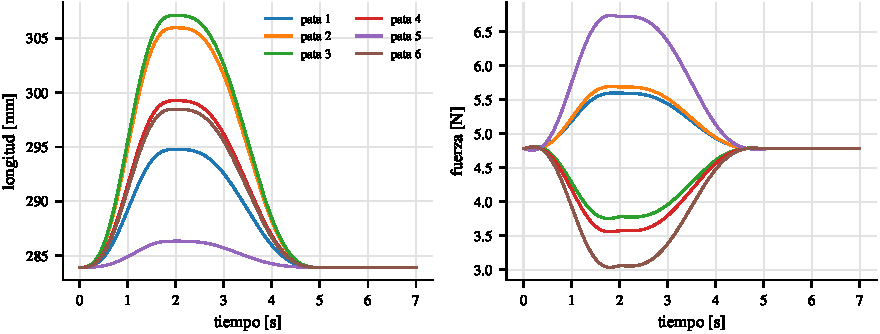
\includegraphics[width=\linewidth]{validacion_modelo.pdf}\\
\fig{Dinámica inversa de la plataforma: longitudes y fuerzas}
\end{columns}
\variables{$g_z$: componente vertical del vector de fuerzas gravitacionales generalizadas [N]; $\vect J_0$: Jacobiano nominal; $\vect F_0$: fuerzas de reposo [N]; $\vect g_0$: vector de fuerzas gravitacionales en la configuración nominal [N, N$\cdot$m]; $F_0$: fuerza de reposo de cada actuador; $0.9509$: componente vertical del vector unitario de cada pata; $\delta\vect F$: desviación de fuerza que maneja el control; $\vect M$: matriz de inercia; $\mathcal V$: energía potencial.}
\end{frame}

% ===================================================================================================

\section{Espacio de estados y linealización}

\begin{frame}{Linealización analítica}
\small
\begin{columns}[T]
\column{0.52\textwidth}
\textbf{Modelo no lineal}, con $\vect x = [\vect q\T\ \dot{\vect q}\T]\T$, $\vect u = \vect F$ y $\vect y = \vect q$:
\[
\dot{\vect x} = \begin{bmatrix}\dot{\vect q}\\ \vect M^{-1}\vect h\end{bmatrix},\qquad \vect h = (\vect J\vect T)\T\vect u + \vect\tau_d - \vect C\dot{\vect q} - \vect g
\]
\textbf{Equilibrio:} $\vect x_0 = [0\ 0\ h_0\ 0\ 0\ 0\ \vect 0]\T$, $\vect u_0 = F_0\vect 1$, $\vect h_0 = \vect 0$

\medskip
\textbf{Derivadas en el equilibrio}
\begin{itemize}
\setlength{\itemsep}{0.2em}
\item Como $\vect h_0 = \vect 0$: \ $\partial(\vect M^{-1}\vect h)/\partial\xi = \vect M_0^{-1}\,\partial\vect h/\partial\xi$
\item $\vect C\dot{\vect q}$ es cuadrático en $\dot{\vect q}$: \ $\partial\vect h/\partial\dot{\vect q} = \vect 0$
\item $\partial\vect h/\partial\vect q = -\vect K_q$, \quad $\partial\vect h/\partial\vect u = \vect J_0\T$
\end{itemize}
\column{0.44\textwidth}
\resultado{$\displaystyle \vect A = \begin{bmatrix}\vect 0 & \vect I\\ \vect A_{21} & \vect 0\end{bmatrix},\qquad \vect B = \begin{bmatrix}\vect 0\\ \vect M_0^{-1}\vect J_0\T\end{bmatrix}$\\[0.4em]
$\vect A_{21} = -\vect M_0^{-1}\vect K_q$}
\textbf{Discretización exacta} con retenedor de orden cero y $T_s = \Ts$ ms:
\[
\exp\!\left(\begin{bmatrix}\vect A & \vect B\\ \vect 0 & \vect 0\end{bmatrix}T_s\right) = \begin{bmatrix}\vect A_d & \vect B_d\\ \vect 0 & \vect I\end{bmatrix}
\]
\end{columns}
\variables{$\vect x$: estado (posición, orientación y velocidades); $\vect u = \vect F$: entrada; $\vect y = \vect q$: salida medida; $\vect h$: fuerza neta; $\vect x_0$, $\vect u_0$: equilibrio; $h_0$: altura nominal; $F_0$: fuerza de reposo; $\xi$: variable respecto a la que se deriva; $\vect K_q$: matriz de rigidez; $\vect A$, $\vect B$: matrices del modelo lineal; $\vect A_{21}$: bloque de rigidez; $\vect M_0$, $\vect J_0$: inercia y Jacobiano nominales; $\vect A_d$, $\vect B_d$: modelo discreto; $T_s$: periodo de muestreo.}
\end{frame}

\begin{frame}{Rigidez geométrica negativa: la plataforma es inestable}
\small
\begin{columns}[T]
\column{0.50\textwidth}
\textbf{Origen.} Con fuerza constante, cada pata aporta la energía $\mathcal V_F = -F_0\,l_i(\vect q)$. Respecto a su extremo $\vect r$:
\begin{align*}
\nabla l_i &= \hat{\vect l}_i,\qquad \nabla^2l_i = \tfrac{1}{l_i}\big(\vect I - \hat{\vect l}_i\hat{\vect l}_i\T\big)\succeq 0\\
\nabla^2\mathcal V_F &= -\tfrac{F_0}{l_i}\big(\vect I - \hat{\vect l}_i\hat{\vect l}_i\T\big)\preceq 0
\end{align*}
Rigidez negativa de $F_0/l_0 = 16.8$ N/m por pata, perpendicular a ella: si el extremo se desplaza de lado, el empuje lo aleja todavía más.
\column{0.46\textwidth}
\textbf{Espectro.} Con $\vect w = [\vect w_1;\ \lambda\vect w_1]$:
\[
\vect A\vect w = \lambda\vect w \;\Rightarrow\; \vect A_{21}\vect w_1 = \lambda^2\vect w_1 \;\Rightarrow\; \lambda = \pm\sqrt\mu
\]
Valores propios de $\vect A_{21}$: $\mu = \{\EigAtwoOne\}$ s$^{-2}$
\resultado{$\lambda(\vect A) = \{\PolosLA\}\ \text{s}^{-1}$}
Seis polos en el semiplano derecho: \textbf{inestable en lazo abierto}. Con fuerzas fijas, una perturbación crece como $e^{\SigmaMax t}$.
\end{columns}
\variables{$\mathcal V_F$: energía potencial de la fuerza constante de una pata; $F_0$: fuerza de reposo; $l_i$: longitud de la pata; $\vect r$: extremo superior de la pata; $\hat{\vect l}_i$: vector unitario; $\nabla$, $\nabla^2$: gradiente y hessiana; $\vect A\vect w = \lambda\vect w$: problema de valores propios; $\mu$: valores propios de $\vect A_{21}$; $\lambda$: polos del modelo lineal [1/s].}
\end{frame}

\begin{frame}{Modelo en las coordenadas de las patas}
\small
Con $\delta\vect l = \vect J_0\delta\vect q$ en $\vect M_0\delta\ddot{\vect q} = \vect J_0\T\delta\vect F - \vect K_q\delta\vect q$, y premultiplicando por $\vect J_0^{-\top}$:
\resultado{$\displaystyle \underbrace{\vect J_0^{-\top}\vect M_0\vect J_0^{-1}}_{\vect\Lambda}\,\delta\ddot{\vect l} = \delta\vect F + \underbrace{\vect J_0^{-\top}\vect M_0\vect A_{21}\vect J_0^{-1}}_{\vect K_l}\,\delta\vect l$}
\begin{columns}[T]
\column{0.48\textwidth}
\textbf{Masa y rigidez vistas por los actuadores}
\begin{itemize}
\setlength{\itemsep}{0.2em}
\item $\lambda(\vect\Lambda) = \{\LamEigs\}$ kg
\item $\lambda(\vect K_l) = \{\KlEigs\}$ N/m, mayor en los giros
\end{itemize}
\column{0.48\textwidth}
\textbf{Consecuencias para el diseño}
\begin{itemize}
\setlength{\itemsep}{0.2em}
\item Con $\delta\vect F = -K_p\delta\vect l$, la rigidez neta es $K_p\vect I - \vect K_l$: \textbf{se necesita} $K_p > \KlMax$ N/m
\item Modelo de una pata: $m = \mLeg$ kg, $k = \kLeg$ N/m
\item Con $T_s = \Ts$ ms (500 Hz) se cubren los modos de lazo cerrado, que superan los 40 rad/s
\end{itemize}
\end{columns}
\variables{$\delta\vect l$: desviación de longitudes; $\delta\vect q$: desviación de posición y orientación; $\vect J_0$: Jacobiano nominal; $\vect M_0$: inercia nominal; $\delta\vect F$: desviación de fuerzas; $\vect K_q$: rigidez en $\vect q$; $\vect\Lambda$: matriz de masa vista por los actuadores; $\vect K_l$: rigidez desestabilizadora en las patas; $K_p$: ganancia proporcional; $m$, $k$: masa y rigidez negativa de una pata; $T_s$: periodo de muestreo.}
\end{frame}

\begin{frame}{Controlabilidad y observabilidad}
\small
\begin{columns}[T]
\column{0.46\textwidth}
\textbf{Observabilidad}, midiendo $\vect y = \vect q$:
\[
\begin{bmatrix}\vect C_y\\ \vect C_y\vect A\end{bmatrix} = \begin{bmatrix}\vect I & \vect 0\\ \vect 0 & \vect I\end{bmatrix}\quad\Rightarrow\quad \mathrm{rank}\,\mathcal O = 12
\]
\textbf{Controlabilidad}, con $\vect B_2 = \vect M_0^{-1}\vect J_0\T$:
\begin{align*}
[\vect B\ \ \vect A\vect B] &= \begin{bmatrix}\vect 0 & \vect B_2\\ \vect B_2 & \vect 0\end{bmatrix}\\
\det[\vect B\ \ \vect A\vect B] &= \pm\det(\vect B_2)^2\\
\det\vect B_2 &= \det(\vect M_0^{-1})\det\vect J_0 \neq 0
\end{align*}
Por lo tanto, $\mathrm{rank}\,\mathcal C = 12$.
\column{0.50\textwidth}
\textbf{Integradores asignables}, sin ceros de transmisión en $s = 0$:
\[
\mathrm{rank}\begin{bmatrix}\vect A & \vect B\\ -\vect C_y & \vect 0\end{bmatrix} = \mathrm{rank}\begin{bmatrix}\vect 0 & \vect I & \vect 0\\ \vect A_{21} & \vect 0 & \vect B_2\\ -\vect I & \vect 0 & \vect 0\end{bmatrix} = 18
\]
\resultado{Sistema controlable y observable en todo el espacio de trabajo; admite acción integral en las seis salidas}
La prueba PBH en los 12 valores propios da el mismo resultado.
\end{columns}
\variables{$\vect C_y = [\vect I\ \vect 0]$: matriz de salida; $\vect A$, $\vect B$: modelo lineal; $\vect A_{21}$: bloque de rigidez; $\vect B_2 = \vect M_0^{-1}\vect J_0\T$; $\mathcal O$, $\mathcal C$: matrices de observabilidad y controlabilidad; PBH: prueba de Popov--Belevitch--Hautus.}
\end{frame}

% ===================================================================================================
\section{Cálculo de variaciones}

\begin{frame}{Euler--Lagrange y condiciones de frontera}
\small
\textbf{Problema.} Encontrar la trayectoria $x^\star(t)$ que minimiza
\[
\mathcal J[x] = \int_{t_0}^{t_f}F(t, x, \dot x)\,dt
\]
\textbf{Primera variación.} Con $x = x^\star + \epsilon\eta$ e integrando por partes:
\[
\delta\mathcal J = \underbrace{F_{\dot x}\big|_{t_f}\eta(t_f) - F_{\dot x}\big|_{t_0}\eta(t_0)}_{\text{términos de los extremos}} + \int_{t_0}^{t_f}\Big(F_x - \tfrac{d}{dt}F_{\dot x}\Big)\eta\,dt = 0
\]
\begin{columns}[T]
\column{0.46\textwidth}
\textbf{En el interior}, por el lema fundamental:
\resultado{$\displaystyle F_x - \frac{d}{dt}F_{\dot x} = 0$}
\column{0.50\textwidth}
\textbf{En cada extremo}
\begin{itemize}
\setlength{\itemsep}{0.3em}
\item \textbf{conocido}: $\eta = 0$ y el término desaparece
\item \textbf{libre}: $\eta$ arbitrario, lo que exige la \textbf{condición natural} $F_{\dot x} = 0$
\end{itemize}
\end{columns}
\variables{$x^\star$: trayectoria óptima; $\mathcal J$: funcional de costo; $F(t, x, \dot x)$: integrando; $F_x$, $F_{\dot x}$: sus derivadas parciales; $\eta$: perturbación de la trayectoria; $\epsilon$: tamaño de la perturbación; $t_0$, $t_f$: instantes inicial y final.}
\end{frame}

\begin{frame}{Casos especiales del integrando: I, II, III y IV}
\small
Según las variables de las que depende $F$, la ecuación de Euler--Lagrange se simplifica:
\begin{center}
\footnotesize
\renewcommand{\arraystretch}{1.55}
\begin{tabular}{@{}clll@{}}
\toprule
Caso & Integrando & Simplificación & Uso en la plataforma \\
\midrule
I & $F(t, \dot x)$, sin $x$ & $F_{\dot x} = c$ & intercepción de la senoidal \\
II & $F(t, x, \dot x)$, con $t$ explícito & sin integral primera & descuento y seguimiento de una onda \\
III & $F(x, \dot x)$, sin $t$ & Beltrami: $\dot xF_{\dot x} - F = C$ & extremos fijos y sus variantes \\
IV & $F(t, x)$, sin $\dot x$ & $F_x = 0$, ecuación algebraica & equilibrio estático \\
\bottomrule
\end{tabular}
\end{center}
\variables{$F$: integrando; $t$: tiempo; $x$, $\dot x$: trayectoria y su derivada; $F_x$, $F_{\dot x}$: derivadas parciales del integrando; $c$, $C$: constantes (integrales primeras).}
\end{frame}

\begin{frame}{Caso I: intercepción de una senoidal}
\begin{columns}[c]
\column{0.55\textwidth}
\small
\textbf{Problema.} Alcanzar $\phi(t) = A\sin\omega t$ desde $z_0 = 5$ mm con el mínimo esfuerzo, $F = \tfrac12\dot z^2$, y $T$ libre.

\textbf{Caso I.} Como $F$ no depende de $z$: $F_{\dot z} = \dot z = c$, así que la trayectoria es una recta, $z = z_0 + ct$.

\textbf{Transversalidad con la curva}
\[
\left[F + F_{\dot z}(\dot\phi - \dot z)\right]_T = c\left(\dot\phi(T) - \tfrac c2\right) = 0
\]
\resultado{$c = 2\dot\phi(T)$, \quad con $z_0 + 2A\omega\cos(\omega T)\,T = A\sin(\omega T)$}
\valores $T = 0.470$ s, $c = 20.35$ mm/s, $z(T) = 14.56$ mm.
\column{0.42\textwidth}
\centering
\begin{tikzpicture}[xscale=2.0,yscale=0.11,font=\scriptsize]
\draw[->] (0,0) -- (2.15,0) node[right]{$t$};
\draw[->] (0,-17) -- (0,19) node[above]{$z$ [mm]};
\draw[gray,thick,domain=0:2.1,samples=80] plot (\x,{15*sin(2*pi*0.45*\x r)});
\draw[red!70!black,thick] (0,5) -- (0.4699,14.56);
\fill[blue!70!black] (0.4699,14.56) circle (0.03 and 0.5);
\node[gray] at (1.5,-12) {$\phi(t)$};
\node[red!70!black] at (0.42,17.5) {$z_0 + ct$};
\end{tikzpicture}\\
\fig{Intercepción óptima de la senoidal}
\end{columns}
\variables{$\phi(t)$: senoidal que se quiere interceptar; $A$, $\omega$: su amplitud y frecuencia; $z_0$: altura inicial; $z(t)$: trayectoria; $F = \tfrac12\dot z^2$: integrando (esfuerzo); $c$: pendiente de la recta óptima [mm/s]; $T$: instante de intercepción.}
\end{frame}

\begin{frame}{Formulación de la maniobra óptima}
\small
\begin{columns}[T]
\column{0.50\textwidth}
\textbf{Problema.} Llevar la plataforma de $q_A$ a $q_B$, con el error normalizado
\[
\varepsilon(t) = \frac{q(t) - q_B}{q_A - q_B},\qquad \varepsilon(0) = 1
\]
\[
\mathcal J[\varepsilon] = \int_0^T\Big(\underbrace{\tfrac12\dot\varepsilon^2}_{\text{esfuerzo}} + \underbrace{\tfrac12a^2\varepsilon^2}_{\text{distancia}}\Big)dt
\]
con $a = 2$ s$^{-1}$ y $T = 2$ s.
\column{0.46\textwidth}
\textbf{Euler--Lagrange}
\[
F_\varepsilon = a^2\varepsilon,\qquad F_{\dot\varepsilon} = \dot\varepsilon,\qquad \tfrac{d}{dt}F_{\dot\varepsilon} = \ddot\varepsilon
\]
\resultado{$\displaystyle \ddot\varepsilon - a^2\varepsilon = 0$}
\[
\varepsilon(t) = C_1\cosh(at) + C_2\sinh(at)
\]
Las condiciones en los extremos fijan $C_1$ y $C_2$.
\end{columns}
\variables{$q_A$, $q_B$: configuraciones inicial y final; $q(t)$: coordenada en el instante $t$; $\varepsilon$: error normalizado respecto al destino; $T$: duración; $a$: peso de la distancia frente al esfuerzo [1/s]; $F_\varepsilon$, $F_{\dot\varepsilon}$: derivadas parciales del integrando; $C_1$, $C_2$: constantes.}
\end{frame}

\begin{frame}{Caso II: descuento exponencial}
\small
\begin{columns}[T]
\column{0.50\textwidth}
Se multiplica el costo de la maniobra por una exponencial decreciente, $L = e^{-\alpha t}F$; el integrando depende explícitamente de $t$:
\[
L_\varepsilon - \tfrac{d}{dt}L_{\dot\varepsilon} = e^{-\alpha t}\left[a^2\varepsilon - \ddot\varepsilon + \alpha\dot\varepsilon\right] = 0
\]
\resultado{$\displaystyle \ddot\varepsilon - \alpha\dot\varepsilon - a^2\varepsilon = 0$}
\[
r_{1,2} = \frac{\alpha\pm\sqrt{\alpha^2 + 4a^2}}{2},\qquad \varepsilon^\star = C_1e^{r_1t} + C_2e^{r_2t}
\]
\column{0.46\textwidth}
\valores con $\alpha = 1$ s$^{-1}$ y extremos fijos
\begin{itemize}
\setlength{\itemsep}{0.2em}
\item $r_1 = 2.5616$, \ $r_2 = -1.5616$ s$^{-1}$
\item $C_1 = -2.62\times10^{-4}$, \ $C_2 = 1.00026$
\item $\varepsilon(1\ \text{s}) = 0.206$
\end{itemize}
El error temprano pesa más que el tardío: la plataforma avanza más despacio al comienzo de la maniobra.
\end{columns}
\variables{$L = e^{-\alpha t}F$: integrando con descuento; $\alpha$: tasa de descuento [1/s]; $L_\varepsilon$, $L_{\dot\varepsilon}$: derivadas parciales; $\varepsilon$: error normalizado; $a$: peso; $r_{1,2}$: raíces características; $C_1$, $C_2$: constantes de la solución.}
\end{frame}

\begin{frame}{Caso III (Beltrami): extremos fijos}
\small
\begin{columns}[T]
\column{0.50\textwidth}
\textbf{Extremos conocidos:} $\varepsilon(0) = 1$ y $\varepsilon(T) = 0$. Con
\[
\varepsilon = D_1\sinh(a(T - t)) + D_2\cosh(a(T - t))
\]
resulta $D_2 = 0$ y $D_1 = 1/\sinh(aT)$.

\textbf{Integral primera (caso III).} Como $F$ no depende de $t$:
\[
\dot\varepsilon F_{\dot\varepsilon} - F = \tfrac12\dot\varepsilon^2 - \tfrac12a^2\varepsilon^2 = C
\]
\textbf{Costo.} Integrando por partes con $\ddot\varepsilon = a^2\varepsilon$:
\[
\mathcal J^\star = \tfrac12\big[\varepsilon\dot\varepsilon\big]_0^T = \tfrac12a\coth(aT)
\]
\column{0.46\textwidth}
\resultado{$\displaystyle \varepsilon^\star(t) = \frac{\sinh(a(T - t))}{\sinh(aT)}$}
\valores
\begin{itemize}
\setlength{\itemsep}{0.2em}
\item $\dot\varepsilon^\star(0) = -a\coth(aT) = -2.0013$ s$^{-1}$
\item $C = a^2/(2\sinh^2(aT)) = 2.69\times10^{-3}$ s$^{-2}$, constante en toda la trayectoria
\item $\mathcal J^\star = 1.00067$ s$^{-1}$; $\varepsilon(1\ \text{s}) = 0.133$, frente a 0.206 con descuento
\item Para $\Delta z = 15$ mm, velocidad inicial de 30 mm/s
\end{itemize}
\end{columns}
\variables{$\varepsilon$: error normalizado; $D_1$, $D_2$: constantes de la solución; $C$: constante de Beltrami; $F$: integrando; $a$: peso; $T$: duración; $\varepsilon^\star$: trayectoria óptima; $\mathcal J^\star$: costo óptimo; $\Delta z$: desplazamiento vertical.}
\end{frame}

\begin{frame}{Caso III: verificación del mínimo}
\small
Euler--Lagrange solo garantiza una trayectoria estacionaria. Tres condiciones confirman el mínimo:
\begin{columns}[T]
\column{0.31\textwidth}
\textbf{Legendre}
\[
F_{\dot\varepsilon\dot\varepsilon} = 1 > 0
\]
condición necesaria de mínimo.
\column{0.31\textwidth}
\textbf{Convexidad}
\[
\vect H_F = \begin{bmatrix}a^2 & 0\\ 0 & 1\end{bmatrix}\succ 0
\]
el mínimo es global.
\column{0.34\textwidth}
\textbf{Ritz}
\[
\varepsilon = \varepsilon^\star + \sum_nb_n\sin\frac{n\pi t}{T}
\]
\[
\mathcal J(b) = \mathcal J^\star + \sum_n\kappa_nb_n^2
\]
\end{columns}
\vspace{0.6em}
\resultado{$\kappa_n = \tfrac T4\big[(n\pi/T)^2 + a^2\big] > 0$: \ $\kappa_1 = 3.234$, $\kappa_2 = 6.935$, $\kappa_3 = 13.10$ s$^{-1}$; toda perturbación aumenta el costo}
\variables{$F_{\dot\varepsilon\dot\varepsilon}$: segunda derivada del integrando respecto a $\dot\varepsilon$; $\vect H_F$: hessiana del integrando; $a$: peso; $b_n$: amplitud del modo $n$ de la perturbación; $T$: duración; $\kappa_n$: coeficiente del modo $n$ en el costo.}
\end{frame}

\begin{frame}{Caso III: estado final libre y tiempo final libre}
\small
Con el mismo integrando del caso III, cada variante libera una condición del problema con extremos fijos:
\begin{center}
\footnotesize
\renewcommand{\arraystretch}{1.5}
\begin{tabular}{@{}L{2.4cm}L{3.3cm}L{3.4cm}L{3.6cm}@{}}
\toprule
Variante & Condición nueva & Trayectoria óptima & Efecto \\
\midrule
Estado final libre & $F_{\dot\varepsilon}(T) = \dot\varepsilon(T) = 0$ & $\varepsilon^\star = \dfrac{\cosh(a(T - t))}{\cosh(aT)}$ & llega en reposo; queda en $\varepsilon(T) = 0.0366$ y $\mathcal J^\star = 0.99933$ \\
Tiempo final libre & $\mathcal H(T) = 0$; por Beltrami, $C = 0$ & $\varepsilon^\star = e^{-at}$ & $\dot\varepsilon = -a\varepsilon$, constante de tiempo de 0.5 s \\
\bottomrule
\end{tabular}
\end{center}
\valores liberar una condición nunca aumenta el costo: con el final libre, $\mathcal J^\star = 0.99933 < 1.00067$ s$^{-1}$.
\variables{$\varepsilon^\star$: trayectoria óptima; $F_{\dot\varepsilon}$: derivada del integrando respecto a $\dot\varepsilon$; $\mathcal H$: hamiltoniano; $C$: constante de Beltrami; $a$: peso; $T$: duración; $\mathcal J^\star$: costo óptimo [1/s].}
\end{frame}

\begin{frame}{Caso IV y caso multivariable}
\small
\textbf{Caso IV.} Si $F$ no depende de $\dot x$, Euler--Lagrange se reduce a $F_x = 0$, una ecuación algebraica: el equilibrio estático $\vect J_0\T\vect F_0 = \vect g_0$, con $F_0 = \Fzero$ N por actuador.

\medskip
\begin{columns}[T]
\column{0.52\textwidth}
\textbf{Caso multivariable:} costo con la inercia de la plataforma
\[
F = \tfrac12\dot{\vect e}\T\vect M_0\dot{\vect e} + \tfrac12\vect e\T\vect K\vect e,\qquad \vect K = a^2\,\mathrm{diag}(\vect M_0)
\]
\textbf{Euler--Lagrange matricial}
\[
\vect M_0\ddot{\vect e} = \vect K\vect e
\quad\Rightarrow\quad
\ddot{\vect e} = \vect W^2\vect e
\]
\[
\vect W^2 = \vect M_0^{-1}\vect K = \vect V\vect\Lambda^2\vect V^{-1}
\]
La solución se descompone en seis modos independientes.
\column{0.44\textwidth}
\resultado{$\displaystyle \vect e^\star(t) = \vect V\,\mathrm{diag}\!\left(\frac{\sinh(\omega_k(T - t))}{\sinh(\omega_kT)}\right)\vect V^{-1}\vect e_0$}
\valores
\begin{itemize}
\setlength{\itemsep}{0.2em}
\item Acoplamiento $x$--$\theta$: $\mu = M_{x\theta}^2/(M_{xx}M_{\theta\theta}) = \muMulti$
\item $\omega_k = \{\omegaMulti\}$ s$^{-1}$, prácticamente iguales a $a$
\item Legendre: $F_{\dot{\vect e}\dot{\vect e}} = \vect M_0\succ 0$
\end{itemize}
\end{columns}
\variables{$\vect J_0$: Jacobiano nominal; $\vect F_0$, $F_0$: fuerzas de reposo; $\vect g_0$: fuerzas gravitacionales nominales; $\vect e$: error respecto al destino; $\vect M_0$: inercia nominal; $\vect K = a^2\,\mathrm{diag}(\vect M_0)$: peso del error; $\vect W^2 = \vect M_0^{-1}\vect K$; $\vect V$, $\vect\Lambda$: vectores y valores propios de $\vect W^2$; $\omega_k$: frecuencia del modo $k$; $M_{x\theta}$: término de acoplamiento de $\vect M_0$; $\mu$: cociente de acoplamiento.}
\end{frame}

\begin{frame}{Casos de frontera A, B, C y D}
\centering
\small
\begin{tabular}{@{}clll@{}}
\toprule
Caso & Inicio $t_0$ & Final $t_f$ & Condiciones \\
\midrule
A & conocido & conocido & $x(t_0) = x_0$, \ $x(t_f) = x_f$ \\
B & conocido & libre & $x(t_0) = x_0$, \ $F_{\dot x}(t_f) = 0$ \\
C & libre & conocido & $F_{\dot x}(t_0) = 0$, \ $x(t_f) = x_f$ \\
D & libre & libre & $F_{\dot x}(t_0) = 0$, \ $F_{\dot x}(t_f) = 0$ \\
\bottomrule
\end{tabular}

\vspace{0.8em}
\begin{columns}[T]
\column{0.48\textwidth}
\begin{block}{Comparación de costos}
Liberar un extremo agrega trayectorias candidatas:
\[
\mathcal J^\star_D \;\le\; \mathcal J^\star_B,\ \mathcal J^\star_C \;\le\; \mathcal J^\star_A
\]
\end{block}
\column{0.48\textwidth}
\begin{block}{¿Por qué una onda?}
Con destino constante, un inicio libre exige $\dot\varepsilon(0) = 0$ y con $\ddot\varepsilon = a^2\varepsilon$ se obtiene $\varepsilon\equiv0$. Para que los cuatro casos tengan sentido se aplican al seguimiento de una onda.
\end{block}
\end{columns}
\variables{$t_0$, $t_f$: instantes inicial y final; $x_0$, $x_f$: valores impuestos en los extremos conocidos; $F_{\dot x}$: derivada del integrando respecto a $\dot x$ (condición natural); $\mathcal J^\star_A, \dots, \mathcal J^\star_D$: costo óptimo de cada caso; $\varepsilon$: error normalizado.}
\end{frame}

\begin{frame}{Casos A--D: seguimiento de una onda (caso II)}
\small
\textbf{Problema.} Reproducir con suavidad una onda en $z$ durante medio periodo:
\[
r(t) = A\cos(\omega t),\qquad A = \AOnda\ \text{mm},\quad \omega = 2\pi\cdot\fOnda = \wOnda\ \text{rad/s}
\]
\[
\mathcal J[x] = \int_0^T\Big(\underbrace{\tfrac12\dot x^2}_{\text{esfuerzo}} + \underbrace{\tfrac12a^2\big(x - r(t)\big)^2}_{\text{distancia a la onda}}\Big)dt,\qquad a = \aOnda\ \text{s}^{-1},\quad T = \TOnda\ \text{s}
\]
\textbf{Euler--Lagrange.} Con $F_x = a^2(x - r)$ y $F_{\dot x} = \dot x$:
\resultado{$\ddot x - a^2x = -a^2r(t)$}
El integrando depende de $t$ a través de la onda (caso II): no hay integral de Beltrami.
\variables{$r(t)$: onda deseada en $z$; $A$, $\omega$: su amplitud y frecuencia; $x(t)$: trayectoria en $z$; $a$: peso del seguimiento [1/s]; $T$: horizonte (medio periodo); $F_x$, $F_{\dot x}$: derivadas parciales del integrando.}
\end{frame}

\begin{frame}{Casos A--D: solución general}
\small
\begin{columns}[T]
\column{0.46\textwidth}
\textbf{Solución particular.} Con $x_p = \kappa r$ y $\ddot r = -\omega^2r$:
\[
-\omega^2\kappa r - a^2\kappa r = -a^2r
\]
\[
\kappa = \frac{a^2}{a^2 + \omega^2} = \kappaOnda
\]
\textbf{Solución general.} Raíces $\pm a$, con $E = e^{-aT} = \EOnda$:
\resultado{$x(t) = \kappa r(t) + C_1e^{-at} + C_2e^{-a(T - t)}$}
\column{0.50\textwidth}
\textbf{Parte homogénea} $h = x - \kappa r$:
\begin{align*}
h(0) &= C_1 + C_2E, & h(T) &= C_1E + C_2\\
\dot h(0) &= -aC_1 + aC_2E, & \dot h(T) &= -aC_1E + aC_2
\end{align*}
\textbf{Extremos}
\begin{itemize}
\item conocido: $x = 0$, es decir, $h = -\kappa r$
\item libre: $\dot x = 0$, es decir, $\dot h = -\kappa\dot r$
\end{itemize}
\valores $r(0) = \rzZero$ mm, $\dot r(0) = \drzZero$ mm/s, $r(T) = \rzT$ mm, $\dot r(T) = \drzT$ mm/s.
\end{columns}
\variables{$x_p$: solución particular; $\kappa$: atenuación de la onda; $r$: onda deseada; $\omega$: su frecuencia; $a$: peso; $E = e^{-aT}$; $C_1$, $C_2$: constantes que corrigen los extremos; $h = x - \kappa r$: parte homogénea; $T$: horizonte.}
\end{frame}

\begin{frame}{Casos A--D: sistemas resueltos (en $z$, mm)}
\small
\begin{align*}
\textbf{A}\ (\text{conocido, conocido}):&\quad C_1 + C_2E = -\kappa r(0),\qquad\ \ C_1E + C_2 = -\kappa r(T)\\
\textbf{B}\ (\text{conocido, libre}):&\quad C_1 + C_2E = -\kappa r(0),\qquad\ \ -aC_1E + aC_2 = -\kappa\dot r(T)\\
\textbf{C}\ (\text{libre, conocido}):&\quad -aC_1 + aC_2E = -\kappa\dot r(0),\quad C_1E + C_2 = -\kappa r(T)\\
\textbf{D}\ (\text{libre, libre}):&\quad -aC_1 + aC_2E = -\kappa\dot r(0),\quad -aC_1E + aC_2 = -\kappa\dot r(T)
\end{align*}
$E$ pequeño: $C_1$ corrige el extremo inferior y $C_2$ el superior (capas límite de $1/a = 0.5$ s); en D, $C_1 = C_2 = 0$ y $x^\star = \kappa r$.

\vspace{0.1em}
\begin{center}
\begin{tabular}{@{}lcccc@{}}
\toprule
 & A & B & C & D \\
\midrule
$C_1$ [mm] & \CUnoA & \CUnoB & \CUnoC & \CUnoD \\
$C_2$ [mm] & \CDosA & \CDosB & \CDosC & \CDosD \\
$z^\star(0)$ [mm] & \xZeroA & \xZeroB & \xZeroC & \xZeroD \\
$z^\star(T)$ [mm] & \xTA & \xTB & \xTC & \xTD \\
$\mathcal J^\star$ [mm$^2$/s] & \JA & \JB & \JC & \JD \\
\bottomrule
\end{tabular}
\end{center}
\variables{$C_1$, $C_2$: constantes de la trayectoria óptima (corrección del extremo inferior y del superior); $E = e^{-aT}$; $\kappa$: atenuación; $r$, $\dot r$: onda deseada y su derivada en los extremos; $a$: peso; $z^\star(0)$, $z^\star(T)$: extremos de la trayectoria óptima; $\mathcal J^\star$: costo óptimo.}
\end{frame}

\begin{frame}{Casos A--D: resultados}
\begin{columns}[c]
\column{0.55\textwidth}
\centering
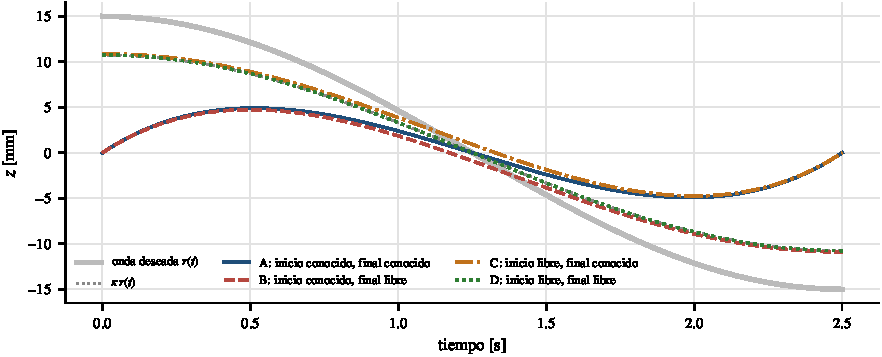
\includegraphics[width=\linewidth]{casos_frontera.pdf}\\
\fig{Casos A--D aplicados a la onda en $z$}
\column{0.42\textwidth}
\small
\begin{itemize}
\setlength{\itemsep}{0.35em}
\item Extremo conocido: la trayectoria llega a cero
\item Extremo libre: pendiente nula; parte o termina en $\kappa r$ (más de 10 mm de diferencia con A)
\item $\mathcal J^\star_D < \mathcal J^\star_B,\ \mathcal J^\star_C < \mathcal J^\star_A$: como predice la inclusión de conjuntos
\item Simulador: posicionamiento en $x^\star(0)$ (extremos fijos, \TPre{} s), trayectoria óptima y regreso
\end{itemize}
\end{columns}
\variables{$\kappa$: atenuación de la onda; $r$: onda deseada; $\mathcal J^\star_A, \dots, \mathcal J^\star_D$: costos óptimos; $F_{\dot x\dot x}$: segunda derivada del integrando (Legendre); $a$: peso; $x^\star(0)$: punto de partida óptimo.}
\end{frame}

% ===================================================================================================
\section{Control óptimo: principio de Pontryagin}

\begin{frame}{Principio del máximo y equivalencia con el cálculo de variaciones}
\small
$\dot{\vect x} = \vect f(\vect x, \vect u)$, $\mathcal J = \int L\,dt$, \ $\mathcal H = L + \vect\lambda\T\vect f$:
\[
\dot{\vect x} = \frac{\partial\mathcal H}{\partial\vect\lambda},\qquad \dot{\vect\lambda} = -\frac{\partial\mathcal H}{\partial\vect x},\qquad \vect u^\star = \arg\min_{\vect u}\mathcal H
\]
El mismo problema con $\dot\varepsilon = u$ y $L = \tfrac12u^2 + \tfrac12a^2\varepsilon^2$:
\[
\mathcal H = \tfrac12u^2 + \tfrac12a^2\varepsilon^2 + \lambda u,\quad u^\star = -\lambda,\quad \dot\lambda = -a^2\varepsilon\ \Rightarrow\ \ddot\varepsilon = -\dot\lambda = a^2\varepsilon
\]
\begin{center}
\footnotesize
\begin{tabular}{@{}ll@{}}
\toprule
Cálculo de variaciones & Pontryagin \\
\midrule
Euler--Lagrange $\ddot\varepsilon = a^2\varepsilon$ & ecuaciones canónicas \\
Beltrami $\dot\varepsilon F_{\dot\varepsilon} - F = C$ & $\mathcal H^\star = -C$ constante \\
Estado final libre $F_{\dot\varepsilon}(T) = 0$ & $\lambda(T) = 0$ \\
Tiempo final libre $[F - \dot\varepsilon F_{\dot\varepsilon}]_T = 0$ & $\mathcal H(T) = 0$ \\
\bottomrule
\end{tabular}
\end{center}
\variables{$\vect x$: estado; $\vect u$: control; $\vect f$: dinámica del sistema; $L$: costo instantáneo; $\mathcal J$: costo total; $\mathcal H$: hamiltoniano; $\vect\lambda$: coestado; $\vect u^\star$: control óptimo; $\varepsilon$: error normalizado; $a$: peso; $C$: constante de Beltrami; $T$: tiempo final.}
\end{frame}

\begin{frame}{Maniobra de mínima energía de una pata}
\small
Pata como doble integrador, $\dot l = v$, $m\dot v = u$, con $m = \mEff$ kg, de reposo a reposo y costo $L = u^2$.

\begin{columns}[T]
\column{0.50\textwidth}
\textbf{Condiciones de Pontryagin}
\begin{align*}
\mathcal H &= u^2 + \lambda_1v + \lambda_2u/m\\
\mathcal H_u &= 0\;\Rightarrow\; u^\star = -\lambda_2/(2m)\\
\dot\lambda_1 &= 0,\ \ \dot\lambda_2 = -\lambda_1\;\Rightarrow\; u^\star = \alpha_0 + \alpha_1t
\end{align*}
\textbf{Fronteras} $v(T) = 0$, $l(T) = \Delta l$:
\[
\alpha_0 = \frac{6m\Delta l}{T^2},\qquad \alpha_1 = -\frac{12m\Delta l}{T^3}
\]
\column{0.46\textwidth}
\resultado{$\displaystyle u^\star(t) = \frac{6m\Delta l}{T^2}\left(1 - \frac{2t}{T}\right)$\\[0.5em]
$\displaystyle E^\star = \frac{12m^2\Delta l^2}{T^3}$}
\[
l(t) = \Delta l\,(3\tau^2 - 2\tau^3),\qquad \tau = t/T
\]
\valores con $\Delta l = \dlEn$ mm y $T = 2$ s: $u^\star(0) = \uEnMax$ mN y $E^\star = \EEn$ N$^2$s.
\end{columns}
\variables{$l$, $v$: elongación y velocidad de la pata; $m$: masa efectiva de la pata [kg]; $u = \delta F$: fuerza de control [N]; $\mathcal H$: hamiltoniano; $\lambda_1$, $\lambda_2$: coestados; $\alpha_0$, $\alpha_1$: coeficientes del control lineal; $\Delta l$: elongación pedida; $T$: duración; $\tau = t/T$; $E^\star$: energía mínima.}
\end{frame}

\begin{frame}{Maniobra de tiempo mínimo: control bang-bang}
\small
Doble integrador con $|\ddot l| \le \ddot l_{\max} = \aMax$ m/s$^2$ y costo de tiempo $L = 1$.
\begin{columns}[T]
\column{0.50\textwidth}
\textbf{Condiciones de Pontryagin}
\begin{align*}
\mathcal H &= 1 + \lambda_1v + \lambda_2\ddot l\\
\ddot l^\star &= -\ddot l_{\max}\,\mathrm{sign}(\lambda_2)\\
\dot\lambda_1 &= 0,\ \ \dot\lambda_2 = -\lambda_1
\end{align*}
$\mathcal H$ es lineal en el control y $\lambda_2$ es una recta: control bang-bang con a lo sumo \textbf{una} conmutación.

\textbf{Simetría} de reposo a reposo: $t_1 = T/2$ y $\tfrac12\Delta l = \tfrac12\ddot l_{\max}t_1^2$.
\column{0.46\textwidth}
\resultado{$\displaystyle T = 2\sqrt{\frac{\Delta l}{\ddot l_{\max}}}$}
\[
l(t) = \begin{cases}\tfrac12\ddot l_{\max}t^2, & t\le T/2\\ \Delta l - \tfrac12\ddot l_{\max}(T - t)^2, & t > T/2\end{cases}
\]
Curva de conmutación: $e = -\dfrac{v|v|}{2\ddot l_{\max}}$

\medskip
\valores con $\Delta l = \dlTm$ mm, $T = \TMin$ s, conmutación en $\tSw$ s, $v_{\max} = \vPico$ mm/s y $m\ddot l_{\max} = \uBang$ mN.
\end{columns}
\variables{$\ddot l$: aceleración de la pata (control); $\ddot l_{\max}$: su límite; $L = 1$: costo de tiempo; $\mathcal H$: hamiltoniano; $\lambda_1$, $\lambda_2$: coestados; $t_1$: instante de conmutación; $\Delta l$: elongación pedida; $T$: tiempo mínimo; $e = l - \Delta l$: error de posición; $v$: velocidad; $v_{\max}$: velocidad máxima; $m$: masa efectiva.}
\end{frame}

% ===================================================================================================
\section{Control PID descentralizado}

\begin{frame}{Modelo de una pata y discretización}
\small
\begin{columns}[T]
\column{0.50\textwidth}
\textbf{Modelo continuo}, diagonal del modelo en las patas:
\[
m\,\delta\ddot l = \delta F + k\,\delta l
\]
\[
G(s) = \frac{1}{ms^2 - k} = \frac{1/m}{(s - \sigma)(s + \sigma)}
\]
con $m = \mLeg$ kg, $k = \kLeg$ N/m y $\sigma = \sqrt{k/m} = \sigmaLeg$ s$^{-1}$.
\textbf{Retenedor de orden cero}, $G(z) = (1 - z^{-1})\,\mathcal Z\{G(s)/s\}$, con
\[
\frac{1}{s(ms^2 - k)} = \frac1k\left[-\frac1s + \frac{1/2}{s - \sigma} + \frac{1/2}{s + \sigma}\right]
\]
\column{0.46\textwidth}
Transformando término a término, con $c = \cosh(\sigma T_s) = \cLeg$:
\resultado{$\displaystyle G(z) = \frac{c - 1}{k}\cdot\frac{z + 1}{z^2 - 2cz + 1}$}
\valores
\begin{itemize}
\setlength{\itemsep}{0.2em}
\item $(c - 1)/k = \gLeg$ m/N
\item Polos $e^{\pm\sigma T_s} = \zUnst$ y $\zSt$
\item Un polo fuera del círculo unitario: la pata es inestable
\end{itemize}
\end{columns}
\variables{$m$: masa vista por la pata [kg]; $k$: rigidez negativa de la pata [N/m]; $\delta l$, $\delta F$: desviaciones de longitud y fuerza; $G(s)$: función de transferencia; $\sigma = \sqrt{k/m}$: polo inestable [1/s]; $G(z)$: función de transferencia discreta; $\mathcal Z$: transformada Z; $c = \cosh(\sigma T_s)$; $T_s$: periodo de muestreo.}
\end{frame}

\begin{frame}{Ley de control discreta}
\small
\resultado{$F_i = F_0 + K_pe_i + K_ix_{I,i} + K_dd_i$}
\begin{columns}[T]
\column{0.54\textwidth}
\textbf{Integral y derivada filtrada}
\begin{align*}
x_{I,i}(k+1) &= x_{I,i}(k) + T_se_i(k)\\
d_i(k) &= \alpha d_i(k-1) + (1 - \alpha)\,\frac{e_i(k) - e_i(k-1)}{T_s}
\end{align*}
\textbf{Función de transferencia}
\[
C(z) = K_p + \frac{K_iT_s}{z - 1} + D\,\frac{z - 1}{z - \alpha},\qquad D = \frac{K_d(1 - \alpha)}{T_s}
\]
Filtro $\alpha = e^{-\omega_fT_s} = \alphaD$ con $\omega_f = 160$ rad/s; anti-\emph{windup} condicional; $|F_i|\le\Fmax$ N.
\column{0.42\textwidth}
\textbf{Ganancias óptimas}
\begin{center}
\footnotesize
\begin{tabular}{@{}lr@{}}
\toprule
$K_p$ & \KpOpt{} N/m \\
$K_i$ & \KiOpt{} N/(m$\cdot$s) \\
$K_d$ & \KdOpt{} N$\cdot$s/m \\
\midrule
$T_i = K_p/K_i$ & \TiOpt{} s \\
$T_d = K_d/K_p$ & \TdOpt{} ms \\
\bottomrule
\end{tabular}
\end{center}
\end{columns}
\variables{$F_i$: fuerza de la pata $i$; $F_0$: fuerza de reposo; $e_i = l_{i,r} - l_i$: error de longitud; $x_{I,i}$: integral del error; $d_i$: derivada filtrada del error; $K_p$, $K_i$, $K_d$: ganancias del PID; $T_s$: periodo de muestreo; $\alpha = e^{-\omega_fT_s}$: polo del filtro; $\omega_f$: frecuencia del filtro derivativo; $D = K_d(1 - \alpha)/T_s$; $C(z)$: controlador discreto; $T_i$, $T_d$: constantes integral y derivativa.}
\end{frame}

\begin{frame}{Condición de estabilidad (Routh)}
\small
$1 + C(s)G(s) = 0$ con $C = K_p + K_i/s + K_ds$, multiplicada por $s(ms^2 - k)$:
\[
ms^3 + K_ds^2 + (K_p - k)s + K_i = 0
\qquad
\begin{array}{c|cc}
s^3 & m & K_p - k\\
s^2 & K_d & K_i\\
s^1 & \frac{K_d(K_p - k) - mK_i}{K_d} & \\
s^0 & K_i &
\end{array}
\qquad\Rightarrow\qquad
\boxed{K_p > k + \frac{mK_i}{K_d}}
\]
\begin{itemize}
\setlength{\itemsep}{0.3em}
\item Sin derivada ($K_d = 0$) es imposible: $K_d$ aporta el amortiguamiento que la planta no tiene
\item $K_p$ debe vencer la rigidez negativa ($k$ y, en MIMO, $\lambda_{\max}(\vect K_l) = \KlMax$ N/m)
\item Óptimo: $K_d(K_p - k) = \RouthL > mK_i = \RouthR$; raíces $\RootsCont$
\end{itemize}
\variables{$C(s)$: PID continuo; $G(s)$: modelo de una pata; $m$: masa; $k$: rigidez negativa; $K_p$, $K_i$, $K_d$: ganancias; $s$: variable de Laplace; $\vect K_l$: rigidez en el espacio de las patas; $\lambda_{\max}$: su mayor valor propio.}
\end{frame}

\begin{frame}{Cruce de ganancia, márgenes y estabilidad}
\begin{columns}[c]
\column{0.56\textwidth}
\small
\textbf{Planta en frecuencia.} Con $s = j\omega$ y el retardo $T_s/2$ del retenedor:
\[
|G| = \frac{1}{m\omega^2 + k},\qquad \angle G = -180^\circ - \frac{\omega T_s}{2}\cdot\frac{180^\circ}{\pi}
\]
La planta está en $-180^\circ$ a toda frecuencia: \textbf{todo el margen lo da la derivada}.

\textbf{Cruce} $|C||G| = 1$ en $\omega_c = \wcHand$ rad/s:
\[
\text{MF} = \angle C - \frac{\omega_cT_s}{2}\cdot\frac{180^\circ}{\pi} = \PMhand^\circ
\]
\resultado{Lazo de una pata con las demás cerradas:\\ MF $= \PMPid^\circ$, \ MG $= \GMPid$ dB, \ $M_s = \MsPid$\\ Lazo completo (30 estados): radio espectral $\rhoPid < 1$}
\column{0.40\textwidth}
\centering
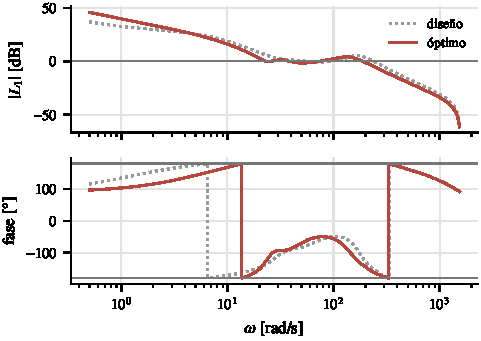
\includegraphics[width=\linewidth]{pid_frecuencia.pdf}\\
\fig{Lazo de una pata con las demás cerradas: PID de diseño y óptimo}
\end{columns}
\variables{$\omega$: frecuencia [rad/s]; $G$, $C$: planta de una pata y PID; $m$, $k$: masa y rigidez negativa; $T_s$: periodo de muestreo; $\omega_c$: frecuencia de cruce de ganancia; MF: margen de fase; MG: margen de ganancia; $M_s$: pico de la sensibilidad.}
\end{frame}

% ===================================================================================================
\section{Realimentación de estados y observador de Luenberger}

\begin{frame}{Sistema aumentado y asignación de polos}
\small
\textbf{Sistema aumentado} con la integral del error $\dot{\vect z} = \vect r - \vect C_y\delta\vect x$:
\[
\begin{bmatrix}\delta\dot{\vect x}\\ \dot{\vect z}\end{bmatrix} = \underbrace{\begin{bmatrix}\vect A & \vect 0\\ -\vect C_y & \vect 0\end{bmatrix}}_{\vect A_a}\begin{bmatrix}\delta\vect x\\ \vect z\end{bmatrix} + \underbrace{\begin{bmatrix}\vect B\\ \vect 0\end{bmatrix}}_{\vect B_a}\delta\vect u,\qquad
\delta\vect u = -\vect K\hat{\vect x} + \vect K_i\vect z + \vect N_r\delta\vect r
\]
\begin{columns}[T]
\column{0.54\textwidth}
\textbf{Asignación por vectores propios.} Para cada polo $\lambda_j$ y dirección de entrada $\vect g_j$:
\[
\vect v_j = (\vect A_a - \lambda_j\vect I)^{-1}\vect B_a\vect g_j
\]
Si $\vect K_a\vect v_j = \vect g_j$, entonces
\[
(\vect A_a - \vect B_a\vect K_a)\vect v_j = \lambda_j\vect v_j
\]
\column{0.42\textwidth}
\resultado{$\vect K_a = \vect G\vect V^{-1}$}
\begin{itemize}
\setlength{\itemsep}{0.2em}
\item Pares conjugados con la misma $\vect g_j$: $\vect K_a$ real
\item Direcciones: columnas normalizadas de $\vect B_2^{-1}$, un eje por par de polos
\end{itemize}
\end{columns}
\variables{$\vect z$: integral del error; $\vect r$: referencia; $\vect C_y$: matriz de salida; $\delta\vect x$: desviación del estado; $\vect A_a$, $\vect B_a$: sistema aumentado; $\delta\vect u$: desviación de fuerzas; $\vect K$, $\vect K_i$: ganancias de estado e integral; $\hat{\vect x}$: estado estimado; $\vect N_r$: precompensador; $\lambda_j$: polo deseado; $\vect g_j$: dirección de entrada; $\vect v_j$: vector propio de lazo cerrado; $\vect K_a = [\vect K\ -\vect K_i]$; $\vect G$, $\vect V$: matrices con las $\vect g_j$ y las $\vect v_j$; $\vect B_2 = \vect M_0^{-1}\vect J_0\T$.}
\end{frame}

\begin{frame}{Polos y precompensador}
\small
\begin{columns}[T]
\column{0.46\textwidth}
\textbf{Polos de diseño}
\begin{itemize}
\setlength{\itemsep}{0.3em}
\item Pares $-25.5 \pm 9j, \dots, -30 \pm 12j$, con $\zeta\approx0.93$ y sobrepaso $< 0.1$~\%
\item Integradores entre $-4.5$ y $-6$
\item Todos a la izquierda de los polos inestables, $+\SigmaMax$
\end{itemize}
\textbf{Óptimo}, escalados por $\alpha = \alphaOpt$:
\begin{itemize}
\item Par dominante $\PoloCtrl$
\item $t_s = 4/\sigma = \tsCtrl$ ms
\end{itemize}
\column{0.50\textwidth}
\textbf{Precompensador.} En régimen, $\vect 0 = (\vect A - \vect B\vect K)\delta\vect x_{ss} + \vect B\vect N_r\delta\vect r$ y $\vect C_y\delta\vect x_{ss} = \delta\vect r$:
\resultado{$\displaystyle \vect N_r = -\left[\vect C_y(\vect A - \vect B\vect K)^{-1}\vect B\right]^{-1}$}
\textbf{Interpretación.} En el equilibrio, con $\delta\vect q = \delta\vect r$:
\[
\vect N_r = \vect K_{pos} - \vect B_2^{-1}\vect A_{21}
\]
compensa la rigidez negativa en la nueva configuración.
\end{columns}
\variables{$\zeta$: amortiguamiento; $\alpha$: factor de escala de los polos; $t_s = 4/\sigma$: tiempo de asentamiento; $\sigma$: parte real del par dominante; $\vect N_r$: precompensador; $\delta\vect x_{ss}$: estado en régimen; $\delta\vect r$: cambio de referencia; $\vect K_{pos}$: parte de $\vect K$ que multiplica la posición y la orientación; $\vect A_{21}$, $\vect B_2$: bloques del modelo lineal.}
\end{frame}

\begin{frame}{Observador de Luenberger: error y dualidad}
\small
Solo se mide $\vect y = \vect q$, y derivarla amplificaría el ruido. El observador es una copia del modelo corregida con la medición:
\resultado{$\dot{\hat{\vect x}} = \vect A\hat{\vect x} + \vect B\vect u + \vect L(\vect y - \vect C_y\hat{\vect x})$}
\begin{columns}[T]
\column{0.50\textwidth}
\textbf{Dinámica del error} $\vect e = \vect x - \hat{\vect x}$:
\[
\dot{\vect e} = (\vect A - \vect L\vect C_y)\,\vect e
\]
No depende de $\vect u$ ni de la referencia; converge si $\vect A - \vect L\vect C_y$ es Hurwitz, y sus polos son asignables porque $(\vect A, \vect C_y)$ es observable.

En la implementación digital se usa el \textbf{estimador actual}: corrige con la medición del mismo instante, sin una muestra de retraso.
\column{0.46\textwidth}
\textbf{Dualidad}
\[
\lambda(\vect A - \vect L\vect C_y) = \lambda\big(\vect A\T - \vect C_y\T\vect L\T\big)
\]
Es una realimentación de estados para $(\vect A\T, \vect C_y\T)$:
\[
\vect L\T = \vect G\vect V^{-1},\qquad \vect v_j = (\vect A\T - \mu_j\vect I)^{-1}\vect C_y\T\vect g_j
\]
\end{columns}
\variables{$\vect y = \vect q$: medición; $\hat{\vect x}$: estado estimado; $\vect L$: ganancia del observador; $\vect C_y$: matriz de salida; $\vect e = \vect x - \hat{\vect x}$: error de estimación; Hurwitz: todos los valores propios en el semiplano izquierdo; $\lambda(\cdot)$: valores propios; $\mu_j$: polos deseados del observador; $\vect g_j$, $\vect v_j$, $\vect G$, $\vect V$: como en la asignación de polos.}
\end{frame}

\begin{frame}{Polos del observador y por qué es más lento}
\small
\begin{columns}[T]
\column{0.46\textwidth}
\textbf{Diseño}
\begin{itemize}
\setlength{\itemsep}{0.3em}
\item $\mu_j^0 = -78\pm18j, \dots, -100.5\pm25.5j$, con $\zeta\approx0.97$
\item Polos discretos $z_j = e^{\beta\mu_j^0T_s}$
\end{itemize}
\textbf{Óptimo}, con $\beta = \betaOpt$:
\begin{itemize}
\setlength{\itemsep}{0.3em}
\item Par dominante $\PoloObs$, \ $|z|_{\max} = \obsZmax$
\item $\vect L_d$ casi diagonal por eje: corrección de posición entre $\LdPos$ y de velocidad entre $\LdVel$ s$^{-1}$
\end{itemize}
\column{0.50\textwidth}
\begin{block}{Compromiso entre ruido y velocidad}
La regla usual, un observador 2 a 5 veces más rápido que el controlador, supone medición sin ruido. Con $\sigma = 0.1$ mm, un $\vect L_d$ grande inyecta el ruido en $\hat{\vect x}$ y, a través de $\vect K$, en las fuerzas de las patas. El ajuste óptimo, que también penaliza el esfuerzo, prefiere un observador más lento que promedie.
\end{block}
\end{columns}
\variables{$\mu_j^0$: polos continuos de diseño del observador; $\zeta$: amortiguamiento; $z_j$: polos discretos; $\beta$: factor de escala de los polos del observador; $T_s$: periodo de muestreo; $\vect L_d$: ganancia del observador; $\sigma$: ruido del sensor; $\vect K$: ganancia del controlador.}
\end{frame}

\begin{frame}{Principio de separación (continuo y discreto)}
\small
\textbf{Continuo.} Con $\vect u = -\vect K\hat{\vect x} = -\vect K(\vect x - \vect e)$:
\[
\begin{bmatrix}\dot{\vect x}\\ \dot{\vect e}\end{bmatrix} = \begin{bmatrix}\vect A - \vect B\vect K & \vect B\vect K\\ \vect 0 & \vect A - \vect L\vect C_y\end{bmatrix}\begin{bmatrix}\vect x\\ \vect e\end{bmatrix}
\quad\Rightarrow\quad
\det(s\vect I - \vect A_{tot}) = \det(s\vect I - \vect A + \vect B\vect K)\,\det(s\vect I - \vect A + \vect L\vect C_y)
\]
\textbf{Discreto}, con integradores y estimador actual:
\[
\begin{bmatrix}\vect x\\ \vect z\\ \vect e_p\end{bmatrix}_{k+1} =
\begin{bmatrix}
\vect A_d - \vect B_d\vect K & \vect B_d\vect K_i & \vect B_d\vect K(\vect I - \vect L_d\vect C_d)\\
-T_s\vect C_d & \vect I & \vect 0\\
\vect 0 & \vect 0 & \vect A_d(\vect I - \vect L_d\vect C_d)
\end{bmatrix}
\begin{bmatrix}\vect x\\ \vect z\\ \vect e_p\end{bmatrix}_k
\]
\resultado{Triangular por bloques: los polos son los del controlador con integradores (radio $\rhoCtrlBlock$) más los del observador (radio $\obsZmax$). Lazo completo: radio espectral $\rhoSS < 1$, estable.}
\variables{$\vect u$: control; $\vect K$: ganancia de estado; $\hat{\vect x}$: estado estimado; $\vect e$: error de estimación; $\vect A_{tot}$: matriz del lazo completo; $\vect L$, $\vect L_d$: ganancias del observador; $\vect C_y$, $\vect C_d$: matrices de salida; $\vect z$: integral del error; $\vect K_i$: ganancia integral; $\vect e_p$: error de predicción; $\vect A_d$, $\vect B_d$: modelo discreto; $T_s$: periodo de muestreo.}
\end{frame}

% ===================================================================================================
\section{Resultados}

\begin{frame}{Comparación (Tabla 1 del protocolo)}
\centering
\small
\begin{tabular}{@{}lcccc@{}}
\toprule
Estrategia & RMS [mm / $^\circ$] & ITAE & $J_u$ [N$^2$s] & Robustez \\
\midrule
\tabinput{../informe/calculos/tablas/tabla1.tex}
\bottomrule
\end{tabular}

\vspace{1.2em}
\begin{columns}[T]
\column{0.45\textwidth}
\begin{block}{PID}
Desempeño comparable en el ensayo, con un modelo mucho más simple.
\end{block}
\column{0.45\textwidth}
\begin{block}{Realimentación de estados}
Mejor en maniobras acopladas y referencias dinámicas; requiere modelo y observador.
\end{block}
\end{columns}
\variables{RMS: error cuadrático medio de posición y de orientación; ITAE: integral del tiempo por el error absoluto; $J_u$: esfuerzo (integral de la fuerza al cuadrado); Robustez: aumento del RMS de posición si la fuerza que entregan los actuadores varía $\pm20$~\% respecto a la comandada.}
\end{frame}

\begin{frame}{Rechazo de perturbaciones e identificación}
\begin{columns}[c]
\column{0.42\textwidth}
\centering
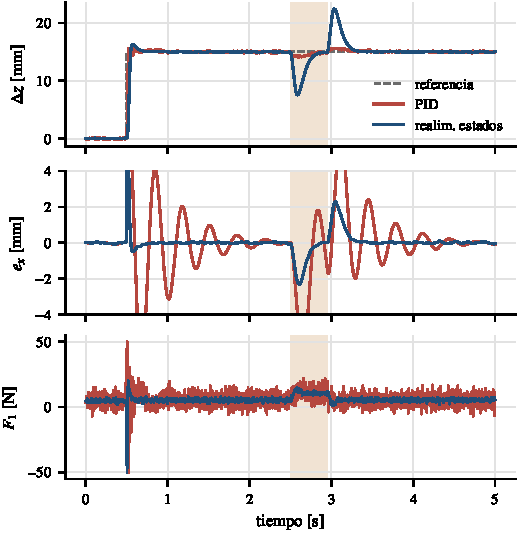
\includegraphics[width=\linewidth,height=0.62\textheight,keepaspectratio]{ensayo_normalizado.pdf}\\
\fig{Ensayo normalizado: escalón e impulso de 20 N}
\column{0.55\textwidth}
\centering
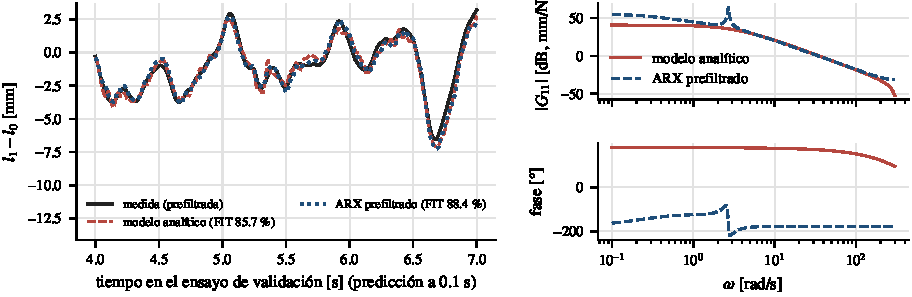
\includegraphics[width=\linewidth]{identificacion.pdf}\\
\fig{Identificación ARX MIMO en lazo cerrado}
\vspace{0.3em}
\small Longitudes con ruido de \IdSigma{} mm y ensayo de validación independiente. ARX directo a \Ts{} ms: sesgado por el ruido en los regresores (masas de \mIdDirMin{} a \mIdDirMax{} kg, FIT \FITunoMedia~\%). Con prefiltro de \IdFc{} Hz y diezmado a \IdTsId{} ms: FIT \FITdosMedia~\% en predicción a \IdHval{} s (analítico: \FITanMedia~\%) y masa de \mIdMin{} a \mIdMax{} kg frente a \mAn{} kg del modelo.
\end{columns}
\end{frame}

\begin{frame}{Gemelo digital}
\begin{columns}[c]
\column{0.62\textwidth}
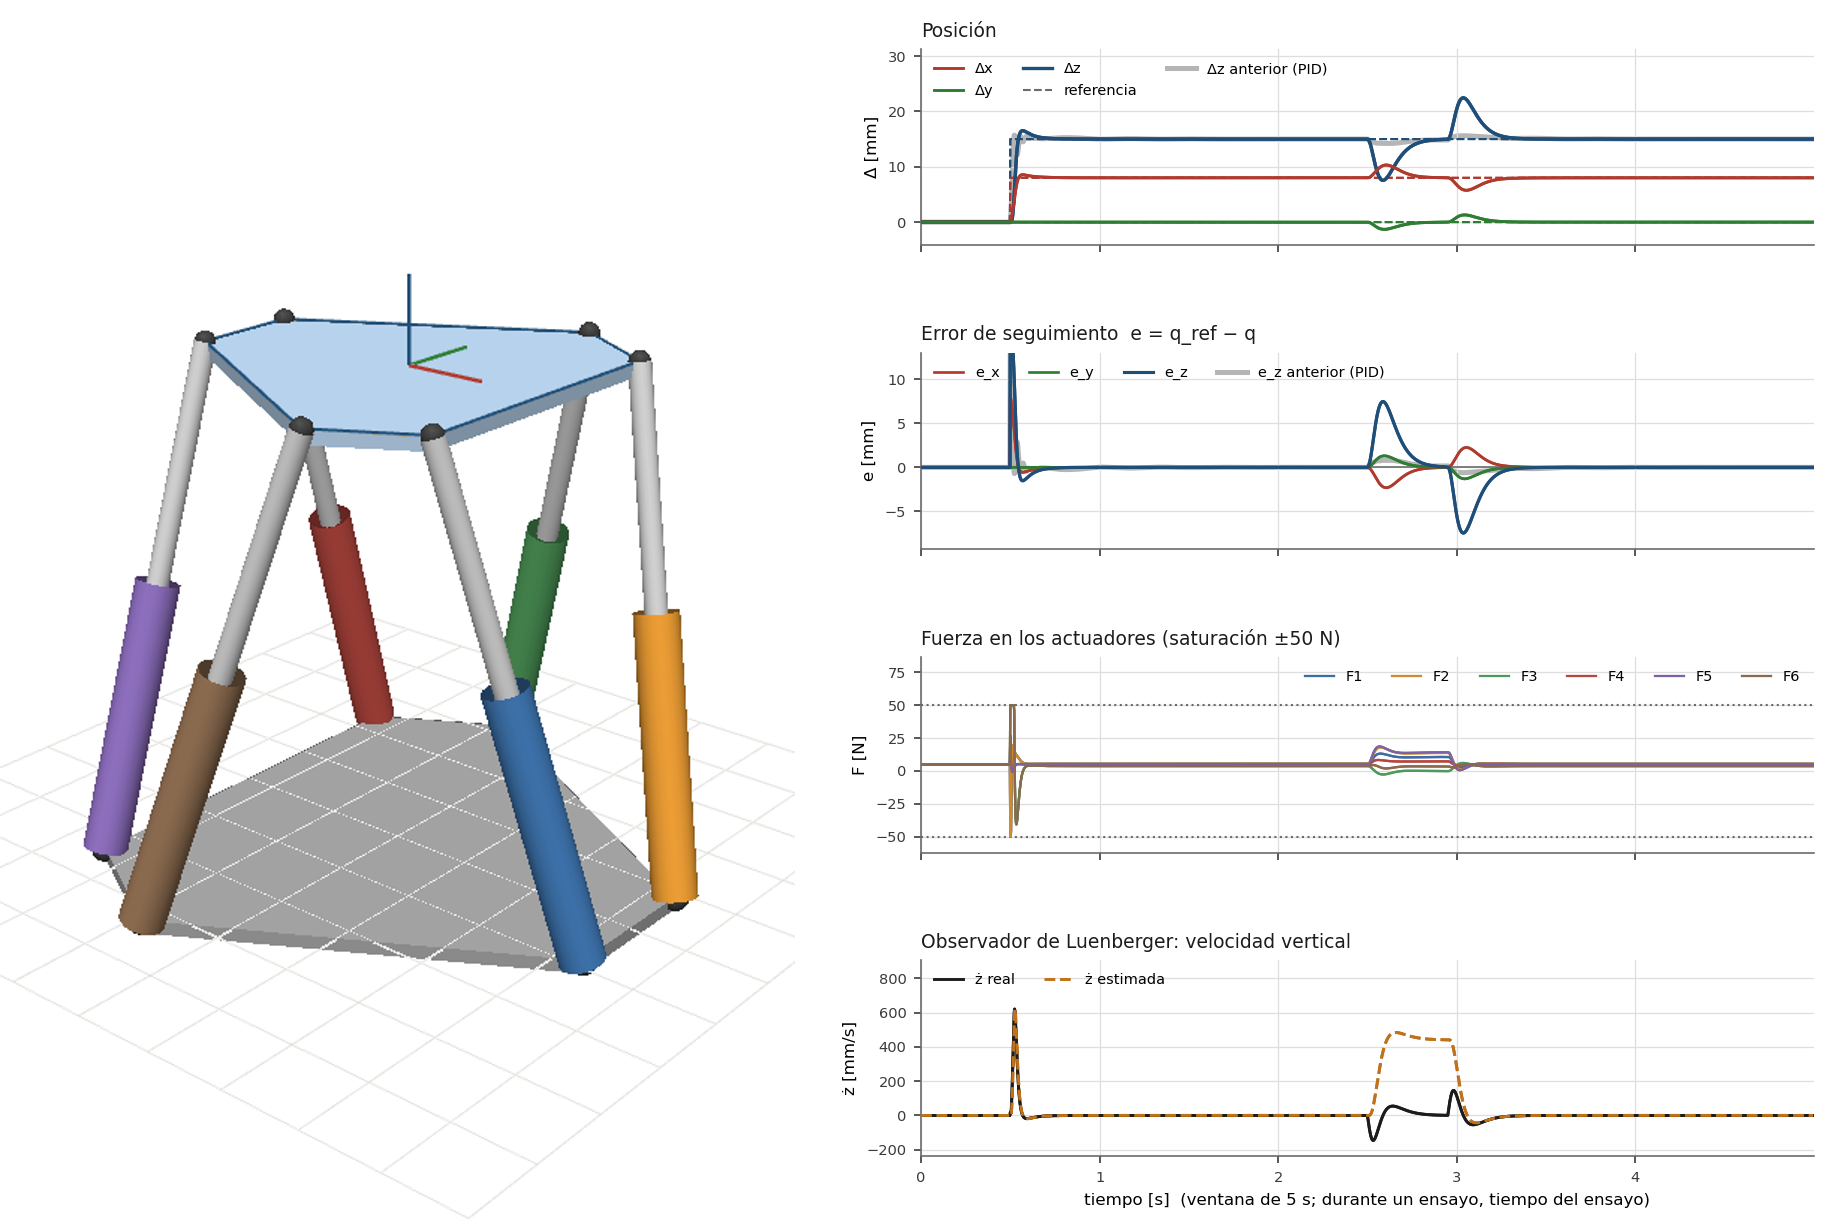
\includegraphics[width=\linewidth]{captura_simulador.png}\\
\fig{Gemelo digital: vista 3D y osciloscopios}
\column{0.34\textwidth}
\small
\begin{itemize}
\setlength{\itemsep}{0.4em}
\item Planta no lineal del modelo analítico; diseño con la linealización
\item Fuerza saturada a $\pm\Fmax$ N, topes y ruido
\item Casos de frontera A--D, trayectorias variacionales y de tiempo mínimo
\item Ganancias óptimas y perturbaciones
\end{itemize}
\end{columns}
\end{frame}

% ===================================================================================================

\begin{frame}{Senoidal en $z$: cálculo y resultado}
\begin{columns}[T]
\column{0.55\textwidth}
\centering
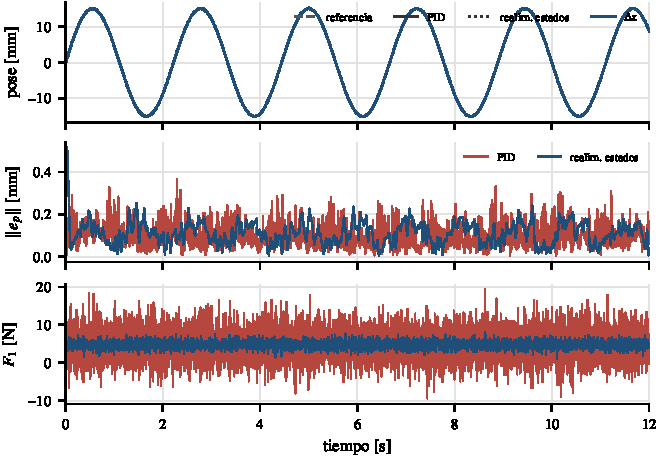
\includegraphics[width=\linewidth,height=0.60\textheight,keepaspectratio]{ref_sine_z.pdf}\\
\fig{Referencia y respuesta de ambas estrategias, norma del error y fuerza de la pata 1}
\column{0.43\textwidth}
\small
\textbf{Cálculo.} $\delta z = 15\sin(2.827t)$ mm: $v_{\max} = A\omega = 42.4$ mm/s, $a_{\max} = A\omega^2 = 119.9$ mm/s$^2$; patas iguales, $\delta l = 0.9509\,\delta z$ (14.26 mm). $\delta F = A(M_{zz}\omega^2 - K_{q,zz})/(6\hat l_z) = 0.098$ N: $F_{ff} = 4.88$ N.

\vspace{0.6em}
\textbf{Resultado.} RMS \RefSenPidRms{} mm (PID) y \RefSenSsRms{} mm (estados): al nivel del ruido. Fuerza simulada \RefSenFreg{} N: el exceso sobre 4.9 N es la respuesta al ruido.
\end{columns}
\variables{$\delta z$: referencia vertical; $A$: amplitud [mm]; $\omega$: frecuencia [rad/s]; $v_{\max}$, $a_{\max}$: velocidad y aceleración máximas; $\delta l$: alargamiento de cada pata; $\hat l_z = 0.9509$: componente vertical del vector unitario de la pata; $\delta F$: fuerza de prealimentación por pata; $M_{zz}$: inercia vertical; $K_{q,zz}$: rigidez vertical; $F_{ff}$: fuerza total.}
\end{frame}

\begin{frame}{Maniobra acoplada de 6 GDL: cálculo y resultado}
\begin{columns}[T]
\column{0.55\textwidth}
\centering
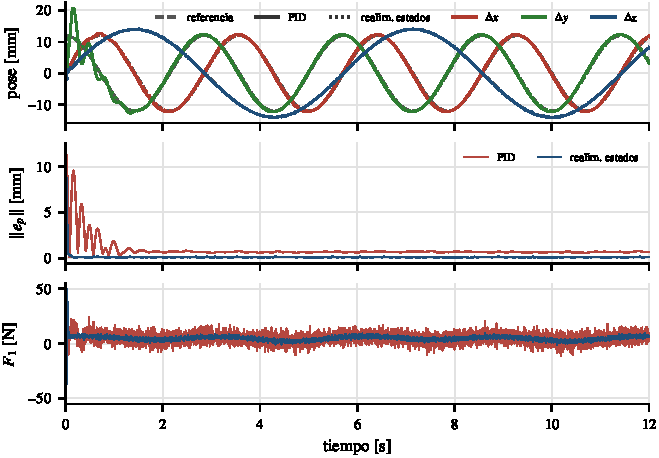
\includegraphics[width=\linewidth,height=0.60\textheight,keepaspectratio]{ref_coupled_6dof.pdf}\\
\fig{Referencia y respuesta de ambas estrategias, norma del error y fuerza de la pata 1}
\column{0.43\textwidth}
\small
\textbf{Cálculo.} $\omega = 2.199$ rad/s; $v_{\max} = \omega\sqrt{12^2 + 7^2} = 30.5$ mm/s, $a \approx 12\omega^2 = 58$ mm/s$^2$; pata más exigida \RefSeisdl{} mm. Arranca en $\delta y = 12$ mm, $\delta\theta = 4.5^\circ$: escalón que satura en $t = 0$.

\vspace{0.6em}
\textbf{Resultado.} RMS \RefSeisPidRms{} mm (PID) frente a \RefSeisSsRms{} mm (estados): el caso que más separa las estrategias, por el acoplamiento traslación--rotación que el PID ve como perturbación.
\end{columns}
\variables{$\omega$: frecuencia de la maniobra [rad/s]; $v_{\max}$: velocidad máxima de traslación; $a$: aceleración; $\delta y$, $\delta\theta$: posición lateral y cabeceo iniciales de la referencia; RMS: error cuadrático medio de posición.}
\end{frame}

\begin{frame}{Trayectoria circular con inclinación: cálculo y resultado}
\begin{columns}[T]
\column{0.55\textwidth}
\centering
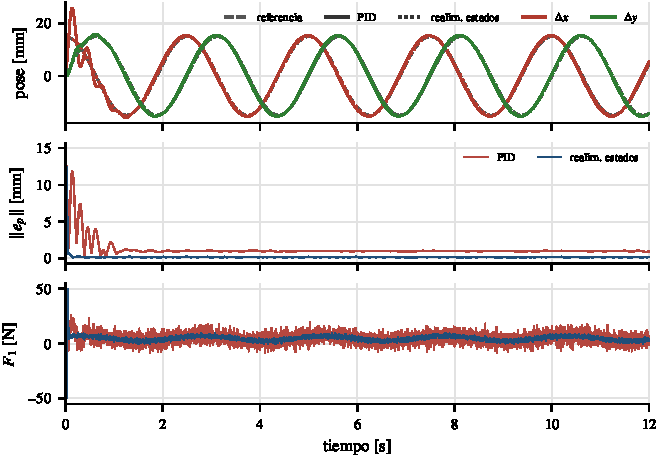
\includegraphics[width=\linewidth,height=0.60\textheight,keepaspectratio]{ref_circle_3d.pdf}\\
\fig{Referencia y respuesta de ambas estrategias, norma del error y fuerza de la pata 1}
\column{0.43\textwidth}
\small
\textbf{Cálculo.} $R = 15$ mm, $\omega = 2.513$ rad/s: $v = R\omega = 37.7$ mm/s y $a = R\omega^2 = 94.8$ mm/s$^2$, constantes; pata más exigida \RefCircdl{} mm; arranque en $\delta x = 15$ mm.

\vspace{0.6em}
\textbf{Resultado.} RMS \RefCircPidRms{} mm (PID) y \RefCircSsRms{} mm (estados); error del PID casi constante: patas en senoides desfasadas y acopladas.
\end{columns}
\variables{$R$: radio del círculo [mm]; $\omega$: velocidad angular del recorrido [rad/s]; $v = R\omega$: velocidad tangencial; $a = R\omega^2$: aceleración centrípeta; $\delta x$: posición inicial de la referencia; RMS: error cuadrático medio de posición.}
\end{frame}

\begin{frame}{Casos de frontera A--D: cálculo y resultados}
\begin{columns}[T]
\column{0.56\textwidth}
\centering
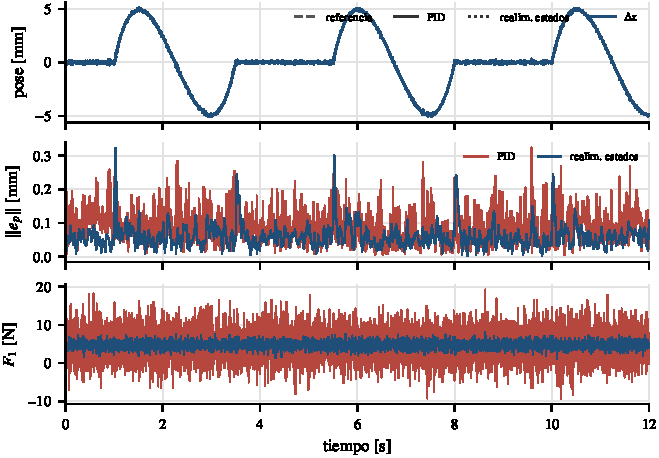
\includegraphics[width=0.49\linewidth]{ref_bc_A.pdf}\hfill
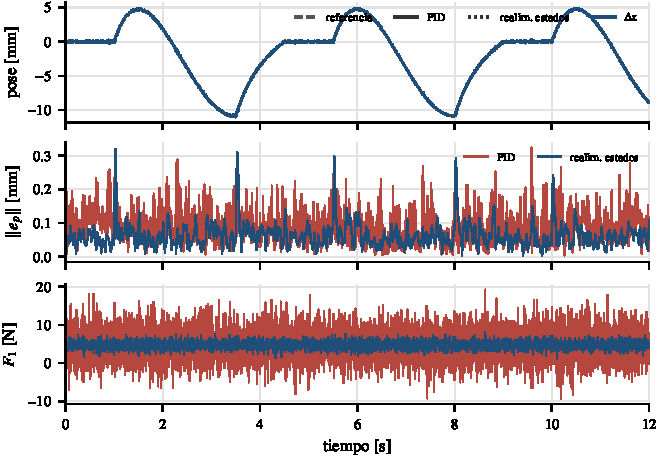
\includegraphics[width=0.49\linewidth]{ref_bc_B.pdf}\\
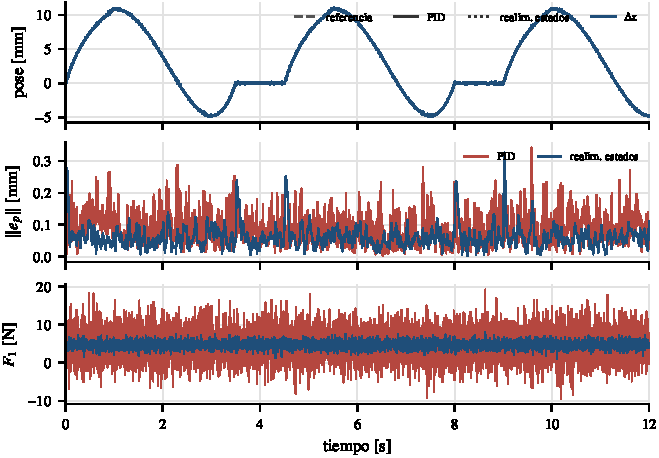
\includegraphics[width=0.49\linewidth]{ref_bc_C.pdf}\hfill
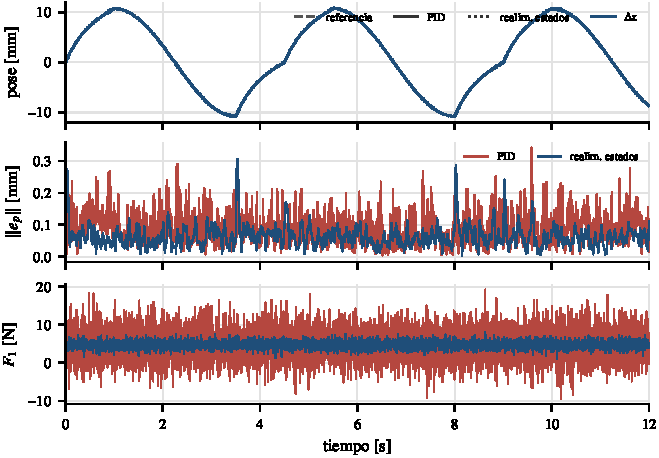
\includegraphics[width=0.49\linewidth]{ref_bc_D.pdf}\\
\fig{Respuesta en $z$ de los casos A, B, C y D}
\column{0.42\textwidth}
\scriptsize
\textbf{Cálculo.} $z^\star = \kappa r + C_1e^{-at} + C_2e^{-a(T-t)}$, $\kappa = \kappaOnda$: A $0\to0$, B $0\to\xTB$, C $\xZeroC\to0$, D $\xZeroD\to\xTD$ mm. $\dot z^\star(0) \ne 0$ en A y B, y el posicionamiento de extremos fijos arranca con $-a\coth(aT)\,\delta z$: saltos de unos 22 mm/s. En los tramos suaves, $\|\ddot{\vect p}\| \le 59$ mm/s$^2$ y $F_{ff} = 4.8$ N.

\textbf{Resultado.} RMS \RefFAPidRms--\RefFDPidRms{} mm (PID) y \RefFASsRms--\RefFDSsRms{} mm (estados); el error máximo (\RefFAPidEmax{} mm) aparece en los saltos de velocidad.
\end{columns}
\variables{$z^\star$: trayectoria óptima en $z$; $\kappa$: atenuación de la onda $r$; $C_1$, $C_2$: constantes de corrección de los extremos; $a$: peso [1/s]; $T$: horizonte; $\|\ddot{\vect p}\|$: aceleración de traslación; $F_{ff}$: fuerza de prealimentación; RMS: error cuadrático medio.}
\end{frame}

\begin{frame}{Maniobra de extremos fijos (Beltrami): cálculo y resultado}
\begin{columns}[T]
\column{0.55\textwidth}
\centering
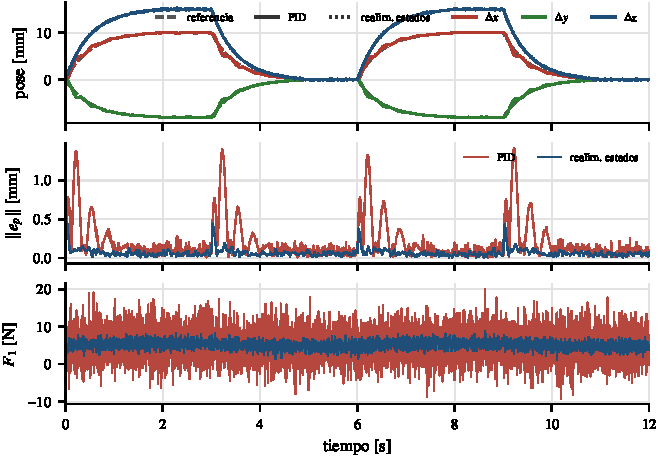
\includegraphics[width=\linewidth,height=0.60\textheight,keepaspectratio]{ref_var_fixed.pdf}\\
\fig{Referencia y respuesta de ambas estrategias, norma del error y fuerza de la pata 1}
\column{0.43\textwidth}
\small
\textbf{Cálculo.} $\|\Delta_p\| = \sqrt{10^2 + 8^2 + 15^2} = 19.72$ mm; $|\dot\varepsilon(0)| = a\coth(aT) = 2.0013$ s$^{-1}$: parte a $19.72\cdot2.0013 = 39.5$ mm/s y llega a $1.4$ mm/s en $t = T$; pata más exigida \RefFijdl{} mm.

\vspace{0.6em}
\textbf{Resultado.} RMS \RefFijPidRms{} mm (PID) y \RefFijSsRms{} mm (estados); errores máximos (\RefFijPidEmax{} y \RefFijSsEmax{} mm) en los arranques.
\end{columns}
\variables{$\Delta_p$: desplazamiento de traslación de la maniobra; $\varepsilon$: error normalizado; $a$: peso [1/s]; $T$: duración; RMS: error cuadrático medio de posición.}
\end{frame}

\begin{frame}{Maniobra de tiempo mínimo (bang-bang): cálculo y resultado}
\begin{columns}[T]
\column{0.55\textwidth}
\centering
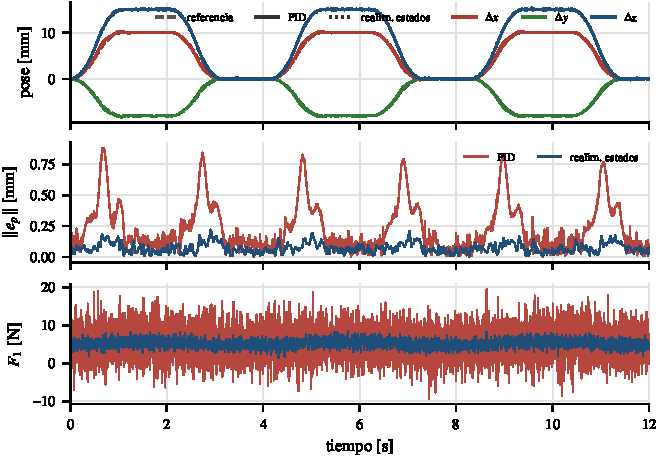
\includegraphics[width=\linewidth,height=0.56\textheight,keepaspectratio]{ref_min_time.pdf}\\
\fig{Referencia y respuesta de ambas estrategias, norma del error y fuerza de la pata 1}
\column{0.43\textwidth}
\small
\textbf{Cálculo.} $\Delta l = \dlTm$ mm, $\ddot l_{\max} = \aMax$ m/s$^2$: $T = 2\sqrt{\Delta l/\ddot l_{\max}} = 1.077$ s, $v_{\max} = \ddot l_{\max}T/2 = 43.1$ mm/s. Parte y llega en reposo: sin saltos de velocidad.

\vspace{0.6em}
\textbf{Resultado.} RMS \RefTminPidRms{} mm (PID) y \RefTminSsRms{} mm (estados): mismo recorrido en la mitad del tiempo, con error parecido al de extremos fijos.
\end{columns}
\variables{$\Delta l$: elongación de la pata más exigida; $\ddot l_{\max}$: aceleración máxima de pata; $T$: tiempo mínimo; $v_{\max}$: velocidad máxima; RMS: error cuadrático medio de posición.}
\end{frame}

\begin{frame}{Síntesis por tipo de movimiento}
\begin{itemize}
\setlength{\itemsep}{0.6em}
\item En los tramos suaves la prealimentación pide de 4.8 a 7.4 N por pata: lejos de los 50 N; la saturación solo aparece en escalones de arranque y en el reinicio de la curva terminal
\item El error crece con la falta de suavidad (saltos de velocidad o de posición), no con la amplitud
\item La realimentación de estados reduce el error entre la mitad y la tercera parte en las maniobras acopladas, y a la cuarta parte en las variacionales y de tiempo mínimo
\item En las referencias verticales simétricas (senoidal, fronteras) ambas estrategias quedan al nivel del ruido
\end{itemize}
\end{frame}

\begin{frame}{Conclusiones}
\small
\begin{enumerate}
\setlength{\itemsep}{0.4em}
\item La rigidez geométrica negativa de las patas hace inestable la plataforma en lazo abierto (polo de 7.62 s$^{-1}$): todo control por pata exige $K_p > 427.8$ N/m y acción derivativa.
\item Las patas aportan el 28\,\% de la inercia de traslación; omitirlas subestima la masa en casi un tercio. La identificación confirma el modelo analítico.
\item El error de seguimiento depende de la suavidad de la referencia y no de su rapidez: la maniobra de tiempo mínimo (1.077 s) tiene el mismo error que la de extremos fijos.
\item Los actuadores tienen holgura: de 4.8 a 7.4 N en tramos suaves frente a 50 N; la saturación solo aparece en los saltos de la referencia.
\item La realimentación de estados es superior en movimientos acoplados: error entre 2.5 y 3 veces menor, 40\,\% menos esfuerzo y menor sensibilidad a los actuadores (23\,\% frente a 29.5\,\%).
\item El PID descentralizado rechaza mejor las perturbaciones (menos de 1 mm ante 20 N) y es suficiente en movimientos verticales, con el modelo de una sola pata.
\item Con ruido de medición, el observador de Luenberger óptimo es más lento que el controlador: el ruido, y no la velocidad, limita su diseño.
\end{enumerate}
\end{frame}

\begin{frame}[plain]
\centering
\vspace*{\fill}
{\color{acento}\Huge\bfseries Gracias}\\[1em]
{\color{tenue}santiago.zuniga-m@mail.escuelaing.edu.co}
\vspace*{\fill}
\end{frame}

\end{document}
